% Created by tikzDevice version 0.12.6 on 2025-02-15 04:40:37
% !TEX encoding = UTF-8 Unicode
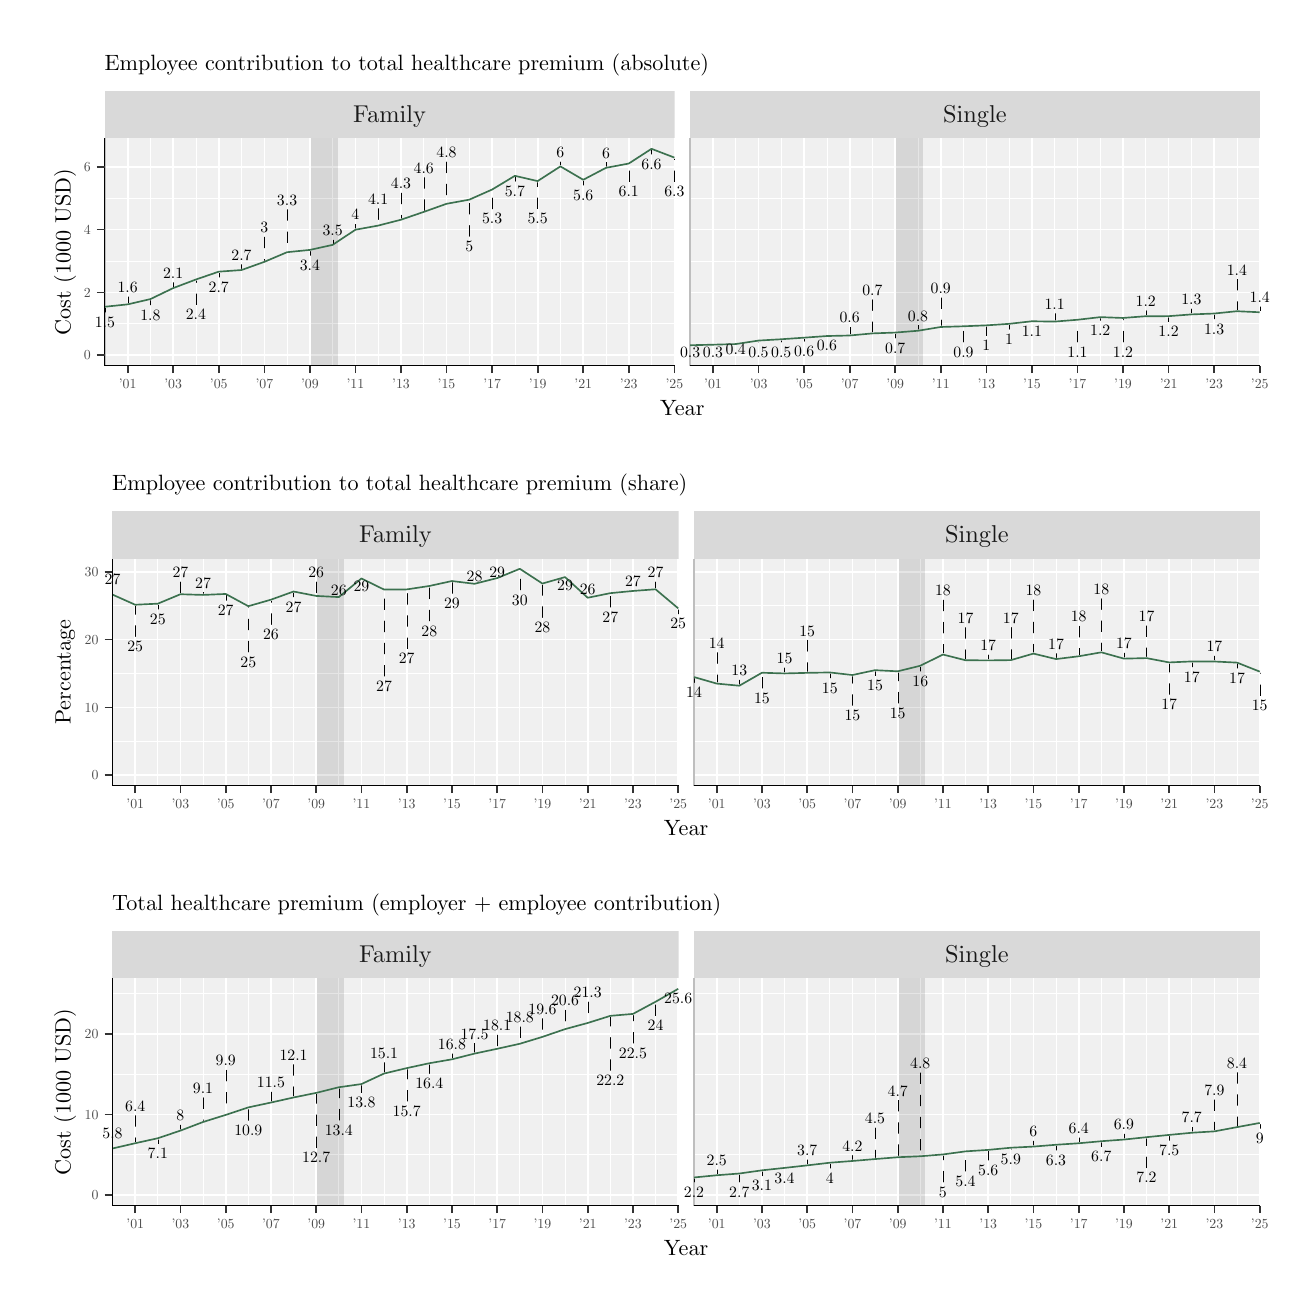
\begin{tikzpicture}[x=1pt,y=1pt]
\definecolor{fillColor}{RGB}{255,255,255}
\path[use as bounding box,fill=fillColor,fill opacity=0.00] (0,0) rectangle (455.30,455.30);
\begin{scope}
\path[clip] (  0.00,303.53) rectangle (455.30,455.30);
\definecolor{drawColor}{RGB}{255,255,255}
\definecolor{fillColor}{RGB}{255,255,255}

\path[draw=drawColor,line width= 0.6pt,line join=round,line cap=round,fill=fillColor] ( -0.00,303.53) rectangle (455.30,455.30);
\end{scope}
\begin{scope}
\path[clip] (  0.00,  0.00) rectangle (455.30,455.30);
\definecolor{fillColor}{gray}{0.94}

\path[fill=fillColor] ( 27.77,333.22) rectangle (233.78,415.25);
\definecolor{drawColor}{RGB}{255,255,255}

\path[draw=drawColor,line width= 0.3pt,line join=round] ( 27.77,348.29) --
	(233.78,348.29);

\path[draw=drawColor,line width= 0.3pt,line join=round] ( 27.77,370.97) --
	(233.78,370.97);

\path[draw=drawColor,line width= 0.3pt,line join=round] ( 27.77,393.66) --
	(233.78,393.66);

\path[draw=drawColor,line width= 0.3pt,line join=round] ( 27.91,333.22) --
	( 27.91,415.25);

\path[draw=drawColor,line width= 0.3pt,line join=round] ( 44.38,333.22) --
	( 44.38,415.25);

\path[draw=drawColor,line width= 0.3pt,line join=round] ( 60.84,333.22) --
	( 60.84,415.25);

\path[draw=drawColor,line width= 0.3pt,line join=round] ( 77.30,333.22) --
	( 77.30,415.25);

\path[draw=drawColor,line width= 0.3pt,line join=round] ( 93.76,333.22) --
	( 93.76,415.25);

\path[draw=drawColor,line width= 0.3pt,line join=round] (110.22,333.22) --
	(110.22,415.25);

\path[draw=drawColor,line width= 0.3pt,line join=round] (126.69,333.22) --
	(126.69,415.25);

\path[draw=drawColor,line width= 0.3pt,line join=round] (143.15,333.22) --
	(143.15,415.25);

\path[draw=drawColor,line width= 0.3pt,line join=round] (159.61,333.22) --
	(159.61,415.25);

\path[draw=drawColor,line width= 0.3pt,line join=round] (176.07,333.22) --
	(176.07,415.25);

\path[draw=drawColor,line width= 0.3pt,line join=round] (192.53,333.22) --
	(192.53,415.25);

\path[draw=drawColor,line width= 0.3pt,line join=round] (209.00,333.22) --
	(209.00,415.25);

\path[draw=drawColor,line width= 0.3pt,line join=round] (225.46,333.22) --
	(225.46,415.25);

\path[draw=drawColor,line width= 0.6pt,line join=round] ( 27.77,336.95) --
	(233.78,336.95);

\path[draw=drawColor,line width= 0.6pt,line join=round] ( 27.77,359.63) --
	(233.78,359.63);

\path[draw=drawColor,line width= 0.6pt,line join=round] ( 27.77,382.32) --
	(233.78,382.32);

\path[draw=drawColor,line width= 0.6pt,line join=round] ( 27.77,405.00) --
	(233.78,405.00);

\path[draw=drawColor,line width= 0.6pt,line join=round] ( 36.15,333.22) --
	( 36.15,415.25);

\path[draw=drawColor,line width= 0.6pt,line join=round] ( 52.60,333.22) --
	( 52.60,415.25);

\path[draw=drawColor,line width= 0.6pt,line join=round] ( 69.07,333.22) --
	( 69.07,415.25);

\path[draw=drawColor,line width= 0.6pt,line join=round] ( 85.52,333.22) --
	( 85.52,415.25);

\path[draw=drawColor,line width= 0.6pt,line join=round] (102.00,333.22) --
	(102.00,415.25);

\path[draw=drawColor,line width= 0.6pt,line join=round] (118.45,333.22) --
	(118.45,415.25);

\path[draw=drawColor,line width= 0.6pt,line join=round] (134.92,333.22) --
	(134.92,415.25);

\path[draw=drawColor,line width= 0.6pt,line join=round] (151.37,333.22) --
	(151.37,415.25);

\path[draw=drawColor,line width= 0.6pt,line join=round] (167.85,333.22) --
	(167.85,415.25);

\path[draw=drawColor,line width= 0.6pt,line join=round] (184.30,333.22) --
	(184.30,415.25);

\path[draw=drawColor,line width= 0.6pt,line join=round] (200.77,333.22) --
	(200.77,415.25);

\path[draw=drawColor,line width= 0.6pt,line join=round] (217.22,333.22) --
	(217.22,415.25);

\path[draw=drawColor,line width= 0.6pt,line join=round] (233.69,333.22) --
	(233.69,415.25);
\definecolor{fillColor}{RGB}{190,190,190}

\path[fill=fillColor,fill opacity=0.01] (102.43,333.22) rectangle (112.05,415.25);

\path[fill=fillColor,fill opacity=0.01] (102.43,333.22) rectangle (112.05,415.25);

\path[fill=fillColor,fill opacity=0.01] (102.43,333.22) rectangle (112.05,415.25);

\path[fill=fillColor,fill opacity=0.01] (102.43,333.22) rectangle (112.05,415.25);

\path[fill=fillColor,fill opacity=0.01] (102.43,333.22) rectangle (112.05,415.25);

\path[fill=fillColor,fill opacity=0.01] (102.43,333.22) rectangle (112.05,415.25);

\path[fill=fillColor,fill opacity=0.01] (102.43,333.22) rectangle (112.05,415.25);

\path[fill=fillColor,fill opacity=0.01] (102.43,333.22) rectangle (112.05,415.25);

\path[fill=fillColor,fill opacity=0.01] (102.43,333.22) rectangle (112.05,415.25);

\path[fill=fillColor,fill opacity=0.01] (102.43,333.22) rectangle (112.05,415.25);

\path[fill=fillColor,fill opacity=0.01] (102.43,333.22) rectangle (112.05,415.25);

\path[fill=fillColor,fill opacity=0.01] (102.43,333.22) rectangle (112.05,415.25);

\path[fill=fillColor,fill opacity=0.01] (102.43,333.22) rectangle (112.05,415.25);

\path[fill=fillColor,fill opacity=0.01] (102.43,333.22) rectangle (112.05,415.25);

\path[fill=fillColor,fill opacity=0.01] (102.43,333.22) rectangle (112.05,415.25);

\path[fill=fillColor,fill opacity=0.01] (102.43,333.22) rectangle (112.05,415.25);

\path[fill=fillColor,fill opacity=0.01] (102.43,333.22) rectangle (112.05,415.25);

\path[fill=fillColor,fill opacity=0.01] (102.43,333.22) rectangle (112.05,415.25);

\path[fill=fillColor,fill opacity=0.01] (102.43,333.22) rectangle (112.05,415.25);

\path[fill=fillColor,fill opacity=0.01] (102.43,333.22) rectangle (112.05,415.25);

\path[fill=fillColor,fill opacity=0.01] (102.43,333.22) rectangle (112.05,415.25);

\path[fill=fillColor,fill opacity=0.01] (102.43,333.22) rectangle (112.05,415.25);

\path[fill=fillColor,fill opacity=0.01] (102.43,333.22) rectangle (112.05,415.25);

\path[fill=fillColor,fill opacity=0.01] (102.43,333.22) rectangle (112.05,415.25);

\path[fill=fillColor,fill opacity=0.01] (102.43,333.22) rectangle (112.05,415.25);

\path[fill=fillColor,fill opacity=0.01] (102.43,333.22) rectangle (112.05,415.25);
\definecolor{drawColor}{RGB}{190,190,190}

\path[draw=drawColor,line width= 0.6pt,line join=round] ( 27.88,333.22) -- ( 27.88,415.25);
\definecolor{drawColor}{RGB}{60,113,79}

\path[draw=drawColor,line width= 0.6pt,line join=round] ( 27.88,354.45) --
	( 36.13,355.31) --
	( 44.35,357.22) --
	( 52.58,361.19) --
	( 60.80,364.30) --
	( 69.05,367.13) --
	( 77.28,367.72) --
	( 85.50,370.67) --
	( 93.73,374.16) --
	(101.98,374.99) --
	(110.20,376.81) --
	(118.43,382.28) --
	(126.65,383.78) --
	(134.90,385.90) --
	(143.12,388.72) --
	(151.35,391.65) --
	(159.58,393.15) --
	(167.82,396.80) --
	(176.05,401.76) --
	(184.27,399.86) --
	(192.50,405.17) --
	(200.75,400.33) --
	(208.97,404.65) --
	(217.20,406.20) --
	(225.42,411.52) --
	(233.67,408.36);
\definecolor{drawColor}{RGB}{0,0,0}

\path[draw=drawColor,line width= 0.1pt,dash pattern=on 4pt off 4pt ,line join=round,line cap=round] ( 27.88,352.44) -- ( 27.88,353.94);

\path[draw=drawColor,line width= 0.1pt,dash pattern=on 4pt off 4pt ,line join=round,line cap=round] ( 36.13,358.05) -- ( 36.13,355.82);

\path[draw=drawColor,line width= 0.1pt,dash pattern=on 4pt off 4pt ,line join=round,line cap=round] ( 44.35,355.05) -- ( 44.35,356.71);

\path[draw=drawColor,line width= 0.1pt,dash pattern=on 4pt off 4pt ,line join=round,line cap=round] ( 52.58,363.21) -- ( 52.58,361.69);

\path[draw=drawColor,line width= 0.1pt,dash pattern=on 4pt off 4pt ,line join=round,line cap=round] ( 60.80,355.16) -- ( 60.80,363.80);

\path[draw=drawColor,line width= 0.1pt,dash pattern=on 4pt off 4pt ,line join=round,line cap=round] ( 69.05,365.10) -- ( 69.05,366.62);

\path[draw=drawColor,line width= 0.1pt,dash pattern=on 4pt off 4pt ,line join=round,line cap=round] ( 77.28,369.75) -- ( 77.28,368.23);

\path[draw=drawColor,line width= 0.1pt,dash pattern=on 4pt off 4pt ,line join=round,line cap=round] ( 85.50,379.64) -- ( 85.50,371.17);

\path[draw=drawColor,line width= 0.1pt,dash pattern=on 4pt off 4pt ,line join=round,line cap=round] ( 93.73,389.58) -- ( 93.73,374.67);

\path[draw=drawColor,line width= 0.1pt,dash pattern=on 4pt off 4pt ,line join=round,line cap=round] (101.98,372.98) -- (101.98,374.48);

\path[draw=drawColor,line width= 0.1pt,dash pattern=on 4pt off 4pt ,line join=round,line cap=round] (110.20,378.55) -- (110.20,377.32);

\path[draw=drawColor,line width= 0.1pt,dash pattern=on 4pt off 4pt ,line join=round,line cap=round] (118.43,384.30) -- (118.43,382.79);

\path[draw=drawColor,line width= 0.1pt,dash pattern=on 4pt off 4pt ,line join=round,line cap=round] (126.65,389.93) -- (126.65,384.29);

\path[draw=drawColor,line width= 0.1pt,dash pattern=on 4pt off 4pt ,line join=round,line cap=round] (134.90,395.56) -- (134.90,386.41);

\path[draw=drawColor,line width= 0.1pt,dash pattern=on 4pt off 4pt ,line join=round,line cap=round] (143.12,401.19) -- (143.12,389.23);

\path[draw=drawColor,line width= 0.1pt,dash pattern=on 4pt off 4pt ,line join=round,line cap=round] (151.35,406.81) -- (151.35,392.16);

\path[draw=drawColor,line width= 0.1pt,dash pattern=on 4pt off 4pt ,line join=round,line cap=round] (159.58,379.86) -- (159.58,392.64);

\path[draw=drawColor,line width= 0.1pt,dash pattern=on 4pt off 4pt ,line join=round,line cap=round] (167.82,389.79) -- (167.82,396.29);

\path[draw=drawColor,line width= 0.1pt,dash pattern=on 4pt off 4pt ,line join=round,line cap=round] (176.05,399.75) -- (176.05,401.25);

\path[draw=drawColor,line width= 0.1pt,dash pattern=on 4pt off 4pt ,line join=round,line cap=round] (184.27,389.83) -- (184.27,399.35);

\path[draw=drawColor,line width= 0.1pt,dash pattern=on 4pt off 4pt ,line join=round,line cap=round] (192.50,406.81) -- (192.50,405.68);

\path[draw=drawColor,line width= 0.1pt,dash pattern=on 4pt off 4pt ,line join=round,line cap=round] (200.75,398.32) -- (200.75,399.82);

\path[draw=drawColor,line width= 0.1pt,dash pattern=on 4pt off 4pt ,line join=round,line cap=round] (208.97,406.68) -- (208.97,405.16);

\path[draw=drawColor,line width= 0.1pt,dash pattern=on 4pt off 4pt ,line join=round,line cap=round] (217.20,399.59) -- (217.20,405.70);

\path[draw=drawColor,line width= 0.1pt,dash pattern=on 4pt off 4pt ,line join=round,line cap=round] (225.42,409.52) -- (225.42,411.01);

\path[draw=drawColor,line width= 0.1pt,dash pattern=on 4pt off 4pt ,line join=round,line cap=round] (233.67,399.58) -- (233.67,407.85);

\node[text=drawColor,anchor=base,inner sep=0pt, outer sep=0pt, scale=  0.57] at ( 27.88,347.01) {1.5};

\node[text=drawColor,anchor=base,inner sep=0pt, outer sep=0pt, scale=  0.57] at ( 36.13,359.56) {1.6};

\node[text=drawColor,anchor=base,inner sep=0pt, outer sep=0pt, scale=  0.57] at ( 44.35,349.62) {1.8};

\node[text=drawColor,anchor=base,inner sep=0pt, outer sep=0pt, scale=  0.57] at ( 52.58,364.72) {2.1};

\node[text=drawColor,anchor=base,inner sep=0pt, outer sep=0pt, scale=  0.57] at ( 60.80,349.73) {2.4};

\node[text=drawColor,anchor=base,inner sep=0pt, outer sep=0pt, scale=  0.57] at ( 69.05,359.68) {2.7};

\node[text=drawColor,anchor=base,inner sep=0pt, outer sep=0pt, scale=  0.57] at ( 77.28,371.25) {2.7};

\node[text=drawColor,anchor=base,inner sep=0pt, outer sep=0pt, scale=  0.57] at ( 85.50,381.14) {3};

\node[text=drawColor,anchor=base,inner sep=0pt, outer sep=0pt, scale=  0.57] at ( 93.73,391.08) {3.3};

\node[text=drawColor,anchor=base,inner sep=0pt, outer sep=0pt, scale=  0.57] at (101.98,367.55) {3.4};

\node[text=drawColor,anchor=base,inner sep=0pt, outer sep=0pt, scale=  0.57] at (110.20,380.06) {3.5};

\node[text=drawColor,anchor=base,inner sep=0pt, outer sep=0pt, scale=  0.57] at (118.43,385.81) {4};

\node[text=drawColor,anchor=base,inner sep=0pt, outer sep=0pt, scale=  0.57] at (126.65,391.44) {4.1};

\node[text=drawColor,anchor=base,inner sep=0pt, outer sep=0pt, scale=  0.57] at (134.90,397.06) {4.3};

\node[text=drawColor,anchor=base,inner sep=0pt, outer sep=0pt, scale=  0.57] at (143.12,402.69) {4.6};

\node[text=drawColor,anchor=base,inner sep=0pt, outer sep=0pt, scale=  0.57] at (151.35,408.32) {4.8};

\node[text=drawColor,anchor=base,inner sep=0pt, outer sep=0pt, scale=  0.57] at (159.58,374.44) {5};

\node[text=drawColor,anchor=base,inner sep=0pt, outer sep=0pt, scale=  0.57] at (167.82,384.37) {5.3};

\node[text=drawColor,anchor=base,inner sep=0pt, outer sep=0pt, scale=  0.57] at (176.05,394.32) {5.7};

\node[text=drawColor,anchor=base,inner sep=0pt, outer sep=0pt, scale=  0.57] at (184.27,384.41) {5.5};

\node[text=drawColor,anchor=base,inner sep=0pt, outer sep=0pt, scale=  0.57] at (192.50,408.32) {6};

\node[text=drawColor,anchor=base,inner sep=0pt, outer sep=0pt, scale=  0.57] at (200.75,392.89) {5.6};

\node[text=drawColor,anchor=base,inner sep=0pt, outer sep=0pt, scale=  0.57] at (208.97,408.19) {6};

\node[text=drawColor,anchor=base,inner sep=0pt, outer sep=0pt, scale=  0.57] at (217.20,394.17) {6.1};

\node[text=drawColor,anchor=base,inner sep=0pt, outer sep=0pt, scale=  0.57] at (225.42,404.09) {6.6};

\node[text=drawColor,anchor=base,inner sep=0pt, outer sep=0pt, scale=  0.57] at (233.67,394.15) {6.3};
\end{scope}
\begin{scope}
\path[clip] (  0.00,  0.00) rectangle (455.30,455.30);
\definecolor{fillColor}{gray}{0.94}

\path[fill=fillColor] (239.28,333.22) rectangle (445.30,415.25);
\definecolor{drawColor}{RGB}{255,255,255}

\path[draw=drawColor,line width= 0.3pt,line join=round] (239.28,348.29) --
	(445.30,348.29);

\path[draw=drawColor,line width= 0.3pt,line join=round] (239.28,370.97) --
	(445.30,370.97);

\path[draw=drawColor,line width= 0.3pt,line join=round] (239.28,393.66) --
	(445.30,393.66);

\path[draw=drawColor,line width= 0.3pt,line join=round] (239.43,333.22) --
	(239.43,415.25);

\path[draw=drawColor,line width= 0.3pt,line join=round] (255.89,333.22) --
	(255.89,415.25);

\path[draw=drawColor,line width= 0.3pt,line join=round] (272.35,333.22) --
	(272.35,415.25);

\path[draw=drawColor,line width= 0.3pt,line join=round] (288.82,333.22) --
	(288.82,415.25);

\path[draw=drawColor,line width= 0.3pt,line join=round] (305.28,333.22) --
	(305.28,415.25);

\path[draw=drawColor,line width= 0.3pt,line join=round] (321.74,333.22) --
	(321.74,415.25);

\path[draw=drawColor,line width= 0.3pt,line join=round] (338.20,333.22) --
	(338.20,415.25);

\path[draw=drawColor,line width= 0.3pt,line join=round] (354.66,333.22) --
	(354.66,415.25);

\path[draw=drawColor,line width= 0.3pt,line join=round] (371.13,333.22) --
	(371.13,415.25);

\path[draw=drawColor,line width= 0.3pt,line join=round] (387.59,333.22) --
	(387.59,415.25);

\path[draw=drawColor,line width= 0.3pt,line join=round] (404.05,333.22) --
	(404.05,415.25);

\path[draw=drawColor,line width= 0.3pt,line join=round] (420.51,333.22) --
	(420.51,415.25);

\path[draw=drawColor,line width= 0.3pt,line join=round] (436.97,333.22) --
	(436.97,415.25);

\path[draw=drawColor,line width= 0.6pt,line join=round] (239.28,336.95) --
	(445.30,336.95);

\path[draw=drawColor,line width= 0.6pt,line join=round] (239.28,359.63) --
	(445.30,359.63);

\path[draw=drawColor,line width= 0.6pt,line join=round] (239.28,382.32) --
	(445.30,382.32);

\path[draw=drawColor,line width= 0.6pt,line join=round] (239.28,405.00) --
	(445.30,405.00);

\path[draw=drawColor,line width= 0.6pt,line join=round] (247.67,333.22) --
	(247.67,415.25);

\path[draw=drawColor,line width= 0.6pt,line join=round] (264.12,333.22) --
	(264.12,415.25);

\path[draw=drawColor,line width= 0.6pt,line join=round] (280.59,333.22) --
	(280.59,415.25);

\path[draw=drawColor,line width= 0.6pt,line join=round] (297.04,333.22) --
	(297.04,415.25);

\path[draw=drawColor,line width= 0.6pt,line join=round] (313.51,333.22) --
	(313.51,415.25);

\path[draw=drawColor,line width= 0.6pt,line join=round] (329.97,333.22) --
	(329.97,415.25);

\path[draw=drawColor,line width= 0.6pt,line join=round] (346.44,333.22) --
	(346.44,415.25);

\path[draw=drawColor,line width= 0.6pt,line join=round] (362.89,333.22) --
	(362.89,415.25);

\path[draw=drawColor,line width= 0.6pt,line join=round] (379.36,333.22) --
	(379.36,415.25);

\path[draw=drawColor,line width= 0.6pt,line join=round] (395.81,333.22) --
	(395.81,415.25);

\path[draw=drawColor,line width= 0.6pt,line join=round] (412.29,333.22) --
	(412.29,415.25);

\path[draw=drawColor,line width= 0.6pt,line join=round] (428.74,333.22) --
	(428.74,415.25);

\path[draw=drawColor,line width= 0.6pt,line join=round] (445.21,333.22) --
	(445.21,415.25);
\definecolor{fillColor}{RGB}{190,190,190}

\path[fill=fillColor,fill opacity=0.01] (313.94,333.22) rectangle (323.57,415.25);

\path[fill=fillColor,fill opacity=0.01] (313.94,333.22) rectangle (323.57,415.25);

\path[fill=fillColor,fill opacity=0.01] (313.94,333.22) rectangle (323.57,415.25);

\path[fill=fillColor,fill opacity=0.01] (313.94,333.22) rectangle (323.57,415.25);

\path[fill=fillColor,fill opacity=0.01] (313.94,333.22) rectangle (323.57,415.25);

\path[fill=fillColor,fill opacity=0.01] (313.94,333.22) rectangle (323.57,415.25);

\path[fill=fillColor,fill opacity=0.01] (313.94,333.22) rectangle (323.57,415.25);

\path[fill=fillColor,fill opacity=0.01] (313.94,333.22) rectangle (323.57,415.25);

\path[fill=fillColor,fill opacity=0.01] (313.94,333.22) rectangle (323.57,415.25);

\path[fill=fillColor,fill opacity=0.01] (313.94,333.22) rectangle (323.57,415.25);

\path[fill=fillColor,fill opacity=0.01] (313.94,333.22) rectangle (323.57,415.25);

\path[fill=fillColor,fill opacity=0.01] (313.94,333.22) rectangle (323.57,415.25);

\path[fill=fillColor,fill opacity=0.01] (313.94,333.22) rectangle (323.57,415.25);

\path[fill=fillColor,fill opacity=0.01] (313.94,333.22) rectangle (323.57,415.25);

\path[fill=fillColor,fill opacity=0.01] (313.94,333.22) rectangle (323.57,415.25);

\path[fill=fillColor,fill opacity=0.01] (313.94,333.22) rectangle (323.57,415.25);

\path[fill=fillColor,fill opacity=0.01] (313.94,333.22) rectangle (323.57,415.25);

\path[fill=fillColor,fill opacity=0.01] (313.94,333.22) rectangle (323.57,415.25);

\path[fill=fillColor,fill opacity=0.01] (313.94,333.22) rectangle (323.57,415.25);

\path[fill=fillColor,fill opacity=0.01] (313.94,333.22) rectangle (323.57,415.25);

\path[fill=fillColor,fill opacity=0.01] (313.94,333.22) rectangle (323.57,415.25);

\path[fill=fillColor,fill opacity=0.01] (313.94,333.22) rectangle (323.57,415.25);

\path[fill=fillColor,fill opacity=0.01] (313.94,333.22) rectangle (323.57,415.25);

\path[fill=fillColor,fill opacity=0.01] (313.94,333.22) rectangle (323.57,415.25);

\path[fill=fillColor,fill opacity=0.01] (313.94,333.22) rectangle (323.57,415.25);

\path[fill=fillColor,fill opacity=0.01] (313.94,333.22) rectangle (323.57,415.25);
\definecolor{drawColor}{RGB}{190,190,190}

\path[draw=drawColor,line width= 0.6pt,line join=round] (239.40,333.22) -- (239.40,415.25);
\definecolor{drawColor}{RGB}{60,113,79}

\path[draw=drawColor,line width= 0.6pt,line join=round] (239.40,340.55) --
	(247.64,340.74) --
	(255.87,340.97) --
	(264.10,342.23) --
	(272.32,342.71) --
	(280.57,343.28) --
	(288.79,343.87) --
	(297.02,344.06) --
	(305.24,344.82) --
	(313.49,345.12) --
	(321.72,345.78) --
	(329.94,347.14) --
	(338.17,347.39) --
	(346.42,347.73) --
	(354.64,348.28) --
	(362.87,349.21) --
	(371.09,349.09) --
	(379.34,349.75) --
	(387.57,350.70) --
	(395.79,350.40) --
	(404.02,351.03) --
	(412.26,351.05) --
	(420.49,351.68) --
	(428.72,352.00) --
	(436.94,352.84) --
	(445.19,352.46);
\definecolor{drawColor}{RGB}{0,0,0}

\path[draw=drawColor,line width= 0.1pt,dash pattern=on 4pt off 4pt ,line join=round,line cap=round] (264.10,341.65) -- (264.10,341.72);

\path[draw=drawColor,line width= 0.1pt,dash pattern=on 4pt off 4pt ,line join=round,line cap=round] (272.32,341.65) -- (272.32,342.20);

\path[draw=drawColor,line width= 0.1pt,dash pattern=on 4pt off 4pt ,line join=round,line cap=round] (280.57,341.92) -- (280.57,342.77);

\path[draw=drawColor,line width= 0.1pt,dash pattern=on 4pt off 4pt ,line join=round,line cap=round] (297.02,347.09) -- (297.02,344.57);

\path[draw=drawColor,line width= 0.1pt,dash pattern=on 4pt off 4pt ,line join=round,line cap=round] (305.24,357.04) -- (305.24,345.33);

\path[draw=drawColor,line width= 0.1pt,dash pattern=on 4pt off 4pt ,line join=round,line cap=round] (313.49,343.11) -- (313.49,344.62);

\path[draw=drawColor,line width= 0.1pt,dash pattern=on 4pt off 4pt ,line join=round,line cap=round] (321.72,347.80) -- (321.72,346.29);

\path[draw=drawColor,line width= 0.1pt,dash pattern=on 4pt off 4pt ,line join=round,line cap=round] (329.94,357.72) -- (329.94,347.65);

\path[draw=drawColor,line width= 0.1pt,dash pattern=on 4pt off 4pt ,line join=round,line cap=round] (338.17,341.65) -- (338.17,346.89);

\path[draw=drawColor,line width= 0.1pt,dash pattern=on 4pt off 4pt ,line join=round,line cap=round] (346.42,343.95) -- (346.42,347.23);

\path[draw=drawColor,line width= 0.1pt,dash pattern=on 4pt off 4pt ,line join=round,line cap=round] (354.64,346.26) -- (354.64,347.77);

\path[draw=drawColor,line width= 0.1pt,dash pattern=on 4pt off 4pt ,line join=round,line cap=round] (371.09,352.02) -- (371.09,349.60);

\path[draw=drawColor,line width= 0.1pt,dash pattern=on 4pt off 4pt ,line join=round,line cap=round] (379.34,341.65) -- (379.34,349.24);

\path[draw=drawColor,line width= 0.1pt,dash pattern=on 4pt off 4pt ,line join=round,line cap=round] (387.57,349.46) -- (387.57,350.20);

\path[draw=drawColor,line width= 0.1pt,dash pattern=on 4pt off 4pt ,line join=round,line cap=round] (395.79,341.65) -- (395.79,349.89);

\path[draw=drawColor,line width= 0.1pt,dash pattern=on 4pt off 4pt ,line join=round,line cap=round] (404.02,353.06) -- (404.02,351.54);

\path[draw=drawColor,line width= 0.1pt,dash pattern=on 4pt off 4pt ,line join=round,line cap=round] (412.26,349.03) -- (412.26,350.54);

\path[draw=drawColor,line width= 0.1pt,dash pattern=on 4pt off 4pt ,line join=round,line cap=round] (420.49,353.69) -- (420.49,352.19);

\path[draw=drawColor,line width= 0.1pt,dash pattern=on 4pt off 4pt ,line join=round,line cap=round] (428.72,349.99) -- (428.72,351.49);

\path[draw=drawColor,line width= 0.1pt,dash pattern=on 4pt off 4pt ,line join=round,line cap=round] (436.94,364.38) -- (436.94,353.34);

\path[draw=drawColor,line width= 0.1pt,dash pattern=on 4pt off 4pt ,line join=round,line cap=round] (445.19,354.48) -- (445.19,352.97);

\node[text=drawColor,anchor=base,inner sep=0pt, outer sep=0pt, scale=  0.57] at (239.40,336.23) {0.3};

\node[text=drawColor,anchor=base,inner sep=0pt, outer sep=0pt, scale=  0.57] at (247.64,336.23) {0.3};

\node[text=drawColor,anchor=base,inner sep=0pt, outer sep=0pt, scale=  0.57] at (255.87,337.13) {0.4};

\node[text=drawColor,anchor=base,inner sep=0pt, outer sep=0pt, scale=  0.57] at (264.10,336.23) {0.5};

\node[text=drawColor,anchor=base,inner sep=0pt, outer sep=0pt, scale=  0.57] at (272.32,336.23) {0.5};

\node[text=drawColor,anchor=base,inner sep=0pt, outer sep=0pt, scale=  0.57] at (280.57,336.50) {0.6};

\node[text=drawColor,anchor=base,inner sep=0pt, outer sep=0pt, scale=  0.57] at (288.79,338.64) {0.6};

\node[text=drawColor,anchor=base,inner sep=0pt, outer sep=0pt, scale=  0.57] at (297.02,348.60) {0.6};

\node[text=drawColor,anchor=base,inner sep=0pt, outer sep=0pt, scale=  0.57] at (305.24,358.55) {0.7};

\node[text=drawColor,anchor=base,inner sep=0pt, outer sep=0pt, scale=  0.57] at (313.49,337.69) {0.7};

\node[text=drawColor,anchor=base,inner sep=0pt, outer sep=0pt, scale=  0.57] at (321.72,349.30) {0.8};

\node[text=drawColor,anchor=base,inner sep=0pt, outer sep=0pt, scale=  0.57] at (329.94,359.23) {0.9};

\node[text=drawColor,anchor=base,inner sep=0pt, outer sep=0pt, scale=  0.57] at (338.17,336.23) {0.9};

\node[text=drawColor,anchor=base,inner sep=0pt, outer sep=0pt, scale=  0.57] at (346.42,338.53) {1};

\node[text=drawColor,anchor=base,inner sep=0pt, outer sep=0pt, scale=  0.57] at (354.64,340.84) {1};

\node[text=drawColor,anchor=base,inner sep=0pt, outer sep=0pt, scale=  0.57] at (362.87,343.61) {1.1};

\node[text=drawColor,anchor=base,inner sep=0pt, outer sep=0pt, scale=  0.57] at (371.09,353.53) {1.1};

\node[text=drawColor,anchor=base,inner sep=0pt, outer sep=0pt, scale=  0.57] at (379.34,336.23) {1.1};

\node[text=drawColor,anchor=base,inner sep=0pt, outer sep=0pt, scale=  0.57] at (387.57,344.04) {1.2};

\node[text=drawColor,anchor=base,inner sep=0pt, outer sep=0pt, scale=  0.57] at (395.79,336.23) {1.2};

\node[text=drawColor,anchor=base,inner sep=0pt, outer sep=0pt, scale=  0.57] at (404.02,354.57) {1.2};

\node[text=drawColor,anchor=base,inner sep=0pt, outer sep=0pt, scale=  0.57] at (412.26,343.61) {1.2};

\node[text=drawColor,anchor=base,inner sep=0pt, outer sep=0pt, scale=  0.57] at (420.49,355.20) {1.3};

\node[text=drawColor,anchor=base,inner sep=0pt, outer sep=0pt, scale=  0.57] at (428.72,344.56) {1.3};

\node[text=drawColor,anchor=base,inner sep=0pt, outer sep=0pt, scale=  0.57] at (436.94,365.88) {1.4};

\node[text=drawColor,anchor=base,inner sep=0pt, outer sep=0pt, scale=  0.57] at (445.19,355.99) {1.4};
\end{scope}
\begin{scope}
\path[clip] ( 27.77,415.25) rectangle (233.78,432.52);
\definecolor{fillColor}{gray}{0.85}

\path[fill=fillColor] ( 27.77,415.25) rectangle (233.78,432.52);
\definecolor{drawColor}{gray}{0.10}

\node[text=drawColor,anchor=base,inner sep=0pt, outer sep=0pt, scale=  0.88] at (130.78,420.86) {Family};
\end{scope}
\begin{scope}
\path[clip] (239.28,415.25) rectangle (445.30,432.52);
\definecolor{fillColor}{gray}{0.85}

\path[fill=fillColor] (239.28,415.25) rectangle (445.30,432.52);
\definecolor{drawColor}{gray}{0.10}

\node[text=drawColor,anchor=base,inner sep=0pt, outer sep=0pt, scale=  0.88] at (342.29,420.86) {Single};
\end{scope}
\begin{scope}
\path[clip] (  0.00,  0.00) rectangle (455.30,455.30);
\definecolor{drawColor}{RGB}{0,0,0}

\path[draw=drawColor,line width= 0.2pt,line join=round] ( 27.77,333.22) --
	(233.78,333.22);
\end{scope}
\begin{scope}
\path[clip] (  0.00,  0.00) rectangle (455.30,455.30);
\definecolor{drawColor}{gray}{0.20}

\path[draw=drawColor,line width= 0.6pt,line join=round] ( 36.15,330.47) --
	( 36.15,333.22);

\path[draw=drawColor,line width= 0.6pt,line join=round] ( 52.60,330.47) --
	( 52.60,333.22);

\path[draw=drawColor,line width= 0.6pt,line join=round] ( 69.07,330.47) --
	( 69.07,333.22);

\path[draw=drawColor,line width= 0.6pt,line join=round] ( 85.52,330.47) --
	( 85.52,333.22);

\path[draw=drawColor,line width= 0.6pt,line join=round] (102.00,330.47) --
	(102.00,333.22);

\path[draw=drawColor,line width= 0.6pt,line join=round] (118.45,330.47) --
	(118.45,333.22);

\path[draw=drawColor,line width= 0.6pt,line join=round] (134.92,330.47) --
	(134.92,333.22);

\path[draw=drawColor,line width= 0.6pt,line join=round] (151.37,330.47) --
	(151.37,333.22);

\path[draw=drawColor,line width= 0.6pt,line join=round] (167.85,330.47) --
	(167.85,333.22);

\path[draw=drawColor,line width= 0.6pt,line join=round] (184.30,330.47) --
	(184.30,333.22);

\path[draw=drawColor,line width= 0.6pt,line join=round] (200.77,330.47) --
	(200.77,333.22);

\path[draw=drawColor,line width= 0.6pt,line join=round] (217.22,330.47) --
	(217.22,333.22);

\path[draw=drawColor,line width= 0.6pt,line join=round] (233.69,330.47) --
	(233.69,333.22);
\end{scope}
\begin{scope}
\path[clip] (  0.00,  0.00) rectangle (455.30,455.30);
\definecolor{drawColor}{gray}{0.30}

\node[text=drawColor,anchor=base,inner sep=0pt, outer sep=0pt, scale=  0.50] at ( 36.15,324.82) {'01};

\node[text=drawColor,anchor=base,inner sep=0pt, outer sep=0pt, scale=  0.50] at ( 52.60,324.82) {'03};

\node[text=drawColor,anchor=base,inner sep=0pt, outer sep=0pt, scale=  0.50] at ( 69.07,324.82) {'05};

\node[text=drawColor,anchor=base,inner sep=0pt, outer sep=0pt, scale=  0.50] at ( 85.52,324.82) {'07};

\node[text=drawColor,anchor=base,inner sep=0pt, outer sep=0pt, scale=  0.50] at (102.00,324.82) {'09};

\node[text=drawColor,anchor=base,inner sep=0pt, outer sep=0pt, scale=  0.50] at (118.45,324.82) {'11};

\node[text=drawColor,anchor=base,inner sep=0pt, outer sep=0pt, scale=  0.50] at (134.92,324.82) {'13};

\node[text=drawColor,anchor=base,inner sep=0pt, outer sep=0pt, scale=  0.50] at (151.37,324.82) {'15};

\node[text=drawColor,anchor=base,inner sep=0pt, outer sep=0pt, scale=  0.50] at (167.85,324.82) {'17};

\node[text=drawColor,anchor=base,inner sep=0pt, outer sep=0pt, scale=  0.50] at (184.30,324.82) {'19};

\node[text=drawColor,anchor=base,inner sep=0pt, outer sep=0pt, scale=  0.50] at (200.77,324.82) {'21};

\node[text=drawColor,anchor=base,inner sep=0pt, outer sep=0pt, scale=  0.50] at (217.22,324.82) {'23};

\node[text=drawColor,anchor=base,inner sep=0pt, outer sep=0pt, scale=  0.50] at (233.69,324.82) {'25};
\end{scope}
\begin{scope}
\path[clip] (  0.00,  0.00) rectangle (455.30,455.30);
\definecolor{drawColor}{RGB}{0,0,0}

\path[draw=drawColor,line width= 0.2pt,line join=round] (239.28,333.22) --
	(445.30,333.22);
\end{scope}
\begin{scope}
\path[clip] (  0.00,  0.00) rectangle (455.30,455.30);
\definecolor{drawColor}{gray}{0.20}

\path[draw=drawColor,line width= 0.6pt,line join=round] (247.67,330.47) --
	(247.67,333.22);

\path[draw=drawColor,line width= 0.6pt,line join=round] (264.12,330.47) --
	(264.12,333.22);

\path[draw=drawColor,line width= 0.6pt,line join=round] (280.59,330.47) --
	(280.59,333.22);

\path[draw=drawColor,line width= 0.6pt,line join=round] (297.04,330.47) --
	(297.04,333.22);

\path[draw=drawColor,line width= 0.6pt,line join=round] (313.51,330.47) --
	(313.51,333.22);

\path[draw=drawColor,line width= 0.6pt,line join=round] (329.97,330.47) --
	(329.97,333.22);

\path[draw=drawColor,line width= 0.6pt,line join=round] (346.44,330.47) --
	(346.44,333.22);

\path[draw=drawColor,line width= 0.6pt,line join=round] (362.89,330.47) --
	(362.89,333.22);

\path[draw=drawColor,line width= 0.6pt,line join=round] (379.36,330.47) --
	(379.36,333.22);

\path[draw=drawColor,line width= 0.6pt,line join=round] (395.81,330.47) --
	(395.81,333.22);

\path[draw=drawColor,line width= 0.6pt,line join=round] (412.29,330.47) --
	(412.29,333.22);

\path[draw=drawColor,line width= 0.6pt,line join=round] (428.74,330.47) --
	(428.74,333.22);

\path[draw=drawColor,line width= 0.6pt,line join=round] (445.21,330.47) --
	(445.21,333.22);
\end{scope}
\begin{scope}
\path[clip] (  0.00,  0.00) rectangle (455.30,455.30);
\definecolor{drawColor}{gray}{0.30}

\node[text=drawColor,anchor=base,inner sep=0pt, outer sep=0pt, scale=  0.50] at (247.67,324.82) {'01};

\node[text=drawColor,anchor=base,inner sep=0pt, outer sep=0pt, scale=  0.50] at (264.12,324.82) {'03};

\node[text=drawColor,anchor=base,inner sep=0pt, outer sep=0pt, scale=  0.50] at (280.59,324.82) {'05};

\node[text=drawColor,anchor=base,inner sep=0pt, outer sep=0pt, scale=  0.50] at (297.04,324.82) {'07};

\node[text=drawColor,anchor=base,inner sep=0pt, outer sep=0pt, scale=  0.50] at (313.51,324.82) {'09};

\node[text=drawColor,anchor=base,inner sep=0pt, outer sep=0pt, scale=  0.50] at (329.97,324.82) {'11};

\node[text=drawColor,anchor=base,inner sep=0pt, outer sep=0pt, scale=  0.50] at (346.44,324.82) {'13};

\node[text=drawColor,anchor=base,inner sep=0pt, outer sep=0pt, scale=  0.50] at (362.89,324.82) {'15};

\node[text=drawColor,anchor=base,inner sep=0pt, outer sep=0pt, scale=  0.50] at (379.36,324.82) {'17};

\node[text=drawColor,anchor=base,inner sep=0pt, outer sep=0pt, scale=  0.50] at (395.81,324.82) {'19};

\node[text=drawColor,anchor=base,inner sep=0pt, outer sep=0pt, scale=  0.50] at (412.29,324.82) {'21};

\node[text=drawColor,anchor=base,inner sep=0pt, outer sep=0pt, scale=  0.50] at (428.74,324.82) {'23};

\node[text=drawColor,anchor=base,inner sep=0pt, outer sep=0pt, scale=  0.50] at (445.21,324.82) {'25};
\end{scope}
\begin{scope}
\path[clip] (  0.00,  0.00) rectangle (455.30,455.30);
\definecolor{drawColor}{RGB}{0,0,0}

\path[draw=drawColor,line width= 0.2pt,line join=round] ( 27.77,333.22) --
	( 27.77,415.25);
\end{scope}
\begin{scope}
\path[clip] (  0.00,  0.00) rectangle (455.30,455.30);
\definecolor{drawColor}{gray}{0.30}

\node[text=drawColor,anchor=base east,inner sep=0pt, outer sep=0pt, scale=  0.50] at ( 22.82,335.22) {0};

\node[text=drawColor,anchor=base east,inner sep=0pt, outer sep=0pt, scale=  0.50] at ( 22.82,357.91) {2};

\node[text=drawColor,anchor=base east,inner sep=0pt, outer sep=0pt, scale=  0.50] at ( 22.82,380.59) {4};

\node[text=drawColor,anchor=base east,inner sep=0pt, outer sep=0pt, scale=  0.50] at ( 22.82,403.28) {6};
\end{scope}
\begin{scope}
\path[clip] (  0.00,  0.00) rectangle (455.30,455.30);
\definecolor{drawColor}{gray}{0.20}

\path[draw=drawColor,line width= 0.6pt,line join=round] ( 25.02,336.95) --
	( 27.77,336.95);

\path[draw=drawColor,line width= 0.6pt,line join=round] ( 25.02,359.63) --
	( 27.77,359.63);

\path[draw=drawColor,line width= 0.6pt,line join=round] ( 25.02,382.32) --
	( 27.77,382.32);

\path[draw=drawColor,line width= 0.6pt,line join=round] ( 25.02,405.00) --
	( 27.77,405.00);
\end{scope}
\begin{scope}
\path[clip] (  0.00,  0.00) rectangle (455.30,455.30);
\definecolor{drawColor}{RGB}{0,0,0}

\node[text=drawColor,anchor=base,inner sep=0pt, outer sep=0pt, scale=  0.80] at (236.53,315.30) {Year};
\end{scope}
\begin{scope}
\path[clip] (  0.00,  0.00) rectangle (455.30,455.30);
\definecolor{drawColor}{RGB}{0,0,0}

\node[text=drawColor,rotate= 90.00,anchor=base,inner sep=0pt, outer sep=0pt, scale=  0.80] at ( 15.51,374.23) {Cost (1000 USD)};
\end{scope}
\begin{scope}
\path[clip] (  0.00,  0.00) rectangle (455.30,455.30);
\definecolor{drawColor}{RGB}{0,0,0}

\node[text=drawColor,anchor=base west,inner sep=0pt, outer sep=0pt, scale=  0.80] at ( 27.77,439.79) {Employee contribution to total healthcare premium (absolute)};
\end{scope}
\begin{scope}
\path[clip] (  0.00,151.77) rectangle (455.30,303.53);
\definecolor{drawColor}{RGB}{255,255,255}
\definecolor{fillColor}{RGB}{255,255,255}

\path[draw=drawColor,line width= 0.6pt,line join=round,line cap=round,fill=fillColor] (  0.00,151.77) rectangle (455.30,303.53);
\end{scope}
\begin{scope}
\path[clip] (  0.00,  0.00) rectangle (455.30,455.30);
\definecolor{fillColor}{gray}{0.94}

\path[fill=fillColor] ( 30.56,181.45) rectangle (235.18,263.48);
\definecolor{drawColor}{RGB}{255,255,255}

\path[draw=drawColor,line width= 0.3pt,line join=round] ( 30.56,197.42) --
	(235.18,197.42);

\path[draw=drawColor,line width= 0.3pt,line join=round] ( 30.56,221.91) --
	(235.18,221.91);

\path[draw=drawColor,line width= 0.3pt,line join=round] ( 30.56,246.40) --
	(235.18,246.40);

\path[draw=drawColor,line width= 0.3pt,line join=round] ( 30.70,181.45) --
	( 30.70,263.48);

\path[draw=drawColor,line width= 0.3pt,line join=round] ( 47.05,181.45) --
	( 47.05,263.48);

\path[draw=drawColor,line width= 0.3pt,line join=round] ( 63.40,181.45) --
	( 63.40,263.48);

\path[draw=drawColor,line width= 0.3pt,line join=round] ( 79.75,181.45) --
	( 79.75,263.48);

\path[draw=drawColor,line width= 0.3pt,line join=round] ( 96.10,181.45) --
	( 96.10,263.48);

\path[draw=drawColor,line width= 0.3pt,line join=round] (112.46,181.45) --
	(112.46,263.48);

\path[draw=drawColor,line width= 0.3pt,line join=round] (128.81,181.45) --
	(128.81,263.48);

\path[draw=drawColor,line width= 0.3pt,line join=round] (145.16,181.45) --
	(145.16,263.48);

\path[draw=drawColor,line width= 0.3pt,line join=round] (161.51,181.45) --
	(161.51,263.48);

\path[draw=drawColor,line width= 0.3pt,line join=round] (177.86,181.45) --
	(177.86,263.48);

\path[draw=drawColor,line width= 0.3pt,line join=round] (194.21,181.45) --
	(194.21,263.48);

\path[draw=drawColor,line width= 0.3pt,line join=round] (210.56,181.45) --
	(210.56,263.48);

\path[draw=drawColor,line width= 0.3pt,line join=round] (226.91,181.45) --
	(226.91,263.48);

\path[draw=drawColor,line width= 0.6pt,line join=round] ( 30.56,185.18) --
	(235.18,185.18);

\path[draw=drawColor,line width= 0.6pt,line join=round] ( 30.56,209.67) --
	(235.18,209.67);

\path[draw=drawColor,line width= 0.6pt,line join=round] ( 30.56,234.16) --
	(235.18,234.16);

\path[draw=drawColor,line width= 0.6pt,line join=round] ( 30.56,258.65) --
	(235.18,258.65);

\path[draw=drawColor,line width= 0.6pt,line join=round] ( 38.88,181.45) --
	( 38.88,263.48);

\path[draw=drawColor,line width= 0.6pt,line join=round] ( 55.22,181.45) --
	( 55.22,263.48);

\path[draw=drawColor,line width= 0.6pt,line join=round] ( 71.58,181.45) --
	( 71.58,263.48);

\path[draw=drawColor,line width= 0.6pt,line join=round] ( 87.92,181.45) --
	( 87.92,263.48);

\path[draw=drawColor,line width= 0.6pt,line join=round] (104.29,181.45) --
	(104.29,263.48);

\path[draw=drawColor,line width= 0.6pt,line join=round] (120.62,181.45) --
	(120.62,263.48);

\path[draw=drawColor,line width= 0.6pt,line join=round] (136.99,181.45) --
	(136.99,263.48);

\path[draw=drawColor,line width= 0.6pt,line join=round] (153.33,181.45) --
	(153.33,263.48);

\path[draw=drawColor,line width= 0.6pt,line join=round] (169.69,181.45) --
	(169.69,263.48);

\path[draw=drawColor,line width= 0.6pt,line join=round] (186.03,181.45) --
	(186.03,263.48);

\path[draw=drawColor,line width= 0.6pt,line join=round] (202.39,181.45) --
	(202.39,263.48);

\path[draw=drawColor,line width= 0.6pt,line join=round] (218.73,181.45) --
	(218.73,263.48);

\path[draw=drawColor,line width= 0.6pt,line join=round] (235.09,181.45) --
	(235.09,263.48);
\definecolor{fillColor}{RGB}{190,190,190}

\path[fill=fillColor,fill opacity=0.01] (104.71,181.45) rectangle (114.27,263.48);

\path[fill=fillColor,fill opacity=0.01] (104.71,181.45) rectangle (114.27,263.48);

\path[fill=fillColor,fill opacity=0.01] (104.71,181.45) rectangle (114.27,263.48);

\path[fill=fillColor,fill opacity=0.01] (104.71,181.45) rectangle (114.27,263.48);

\path[fill=fillColor,fill opacity=0.01] (104.71,181.45) rectangle (114.27,263.48);

\path[fill=fillColor,fill opacity=0.01] (104.71,181.45) rectangle (114.27,263.48);

\path[fill=fillColor,fill opacity=0.01] (104.71,181.45) rectangle (114.27,263.48);

\path[fill=fillColor,fill opacity=0.01] (104.71,181.45) rectangle (114.27,263.48);

\path[fill=fillColor,fill opacity=0.01] (104.71,181.45) rectangle (114.27,263.48);

\path[fill=fillColor,fill opacity=0.01] (104.71,181.45) rectangle (114.27,263.48);

\path[fill=fillColor,fill opacity=0.01] (104.71,181.45) rectangle (114.27,263.48);

\path[fill=fillColor,fill opacity=0.01] (104.71,181.45) rectangle (114.27,263.48);

\path[fill=fillColor,fill opacity=0.01] (104.71,181.45) rectangle (114.27,263.48);

\path[fill=fillColor,fill opacity=0.01] (104.71,181.45) rectangle (114.27,263.48);

\path[fill=fillColor,fill opacity=0.01] (104.71,181.45) rectangle (114.27,263.48);

\path[fill=fillColor,fill opacity=0.01] (104.71,181.45) rectangle (114.27,263.48);

\path[fill=fillColor,fill opacity=0.01] (104.71,181.45) rectangle (114.27,263.48);

\path[fill=fillColor,fill opacity=0.01] (104.71,181.45) rectangle (114.27,263.48);

\path[fill=fillColor,fill opacity=0.01] (104.71,181.45) rectangle (114.27,263.48);

\path[fill=fillColor,fill opacity=0.01] (104.71,181.45) rectangle (114.27,263.48);

\path[fill=fillColor,fill opacity=0.01] (104.71,181.45) rectangle (114.27,263.48);

\path[fill=fillColor,fill opacity=0.01] (104.71,181.45) rectangle (114.27,263.48);

\path[fill=fillColor,fill opacity=0.01] (104.71,181.45) rectangle (114.27,263.48);

\path[fill=fillColor,fill opacity=0.01] (104.71,181.45) rectangle (114.27,263.48);

\path[fill=fillColor,fill opacity=0.01] (104.71,181.45) rectangle (114.27,263.48);

\path[fill=fillColor,fill opacity=0.01] (104.71,181.45) rectangle (114.27,263.48);
\definecolor{drawColor}{RGB}{190,190,190}

\path[draw=drawColor,line width= 0.6pt,line join=round] ( 30.67,181.45) -- ( 30.67,263.48);
\definecolor{drawColor}{RGB}{60,113,79}

\path[draw=drawColor,line width= 0.6pt,line join=round] ( 30.67,250.43) --
	( 38.86,246.77) --
	( 47.03,247.16) --
	( 55.20,250.57) --
	( 63.37,250.32) --
	( 71.56,250.67) --
	( 79.73,246.25) --
	( 87.90,248.60) --
	( 96.07,251.55) --
	(104.26,249.96) --
	(112.43,249.54) --
	(120.60,256.27) --
	(128.77,252.26) --
	(136.96,252.31) --
	(145.13,253.55) --
	(153.30,255.34) --
	(161.47,254.34) --
	(169.67,256.41) --
	(177.83,259.76) --
	(186.00,254.43) --
	(194.17,256.77) --
	(202.37,249.30) --
	(210.54,250.96) --
	(218.71,251.75) --
	(226.88,252.36) --
	(235.07,245.47);
\definecolor{drawColor}{RGB}{0,0,0}

\path[draw=drawColor,line width= 0.1pt,dash pattern=on 4pt off 4pt ,line join=round,line cap=round] ( 30.67,252.44) -- ( 30.67,250.94);

\path[draw=drawColor,line width= 0.1pt,dash pattern=on 4pt off 4pt ,line join=round,line cap=round] ( 38.86,235.25) -- ( 38.86,246.25);

\path[draw=drawColor,line width= 0.1pt,dash pattern=on 4pt off 4pt ,line join=round,line cap=round] ( 47.03,245.13) -- ( 47.03,246.65);

\path[draw=drawColor,line width= 0.1pt,dash pattern=on 4pt off 4pt ,line join=round,line cap=round] ( 55.20,255.05) -- ( 55.20,251.08);

\path[draw=drawColor,line width= 0.1pt,dash pattern=on 4pt off 4pt ,line join=round,line cap=round] ( 63.37,251.27) -- ( 63.37,250.83);

\path[draw=drawColor,line width= 0.1pt,dash pattern=on 4pt off 4pt ,line join=round,line cap=round] ( 71.56,248.28) -- ( 71.56,250.16);

\path[draw=drawColor,line width= 0.1pt,dash pattern=on 4pt off 4pt ,line join=round,line cap=round] ( 79.73,229.65) -- ( 79.73,245.74);

\path[draw=drawColor,line width= 0.1pt,dash pattern=on 4pt off 4pt ,line join=round,line cap=round] ( 87.90,239.59) -- ( 87.90,248.09);

\path[draw=drawColor,line width= 0.1pt,dash pattern=on 4pt off 4pt ,line join=round,line cap=round] ( 96.07,249.53) -- ( 96.07,251.04);

\path[draw=drawColor,line width= 0.1pt,dash pattern=on 4pt off 4pt ,line join=round,line cap=round] (104.26,255.05) -- (104.26,250.47);

\path[draw=drawColor,line width= 0.1pt,dash pattern=on 4pt off 4pt ,line join=round,line cap=round] (128.77,220.94) -- (128.77,251.75);

\path[draw=drawColor,line width= 0.1pt,dash pattern=on 4pt off 4pt ,line join=round,line cap=round] (136.96,230.88) -- (136.96,251.80);

\path[draw=drawColor,line width= 0.1pt,dash pattern=on 4pt off 4pt ,line join=round,line cap=round] (145.13,240.89) -- (145.13,253.04);

\path[draw=drawColor,line width= 0.1pt,dash pattern=on 4pt off 4pt ,line join=round,line cap=round] (153.30,250.80) -- (153.30,254.83);

\path[draw=drawColor,line width= 0.1pt,dash pattern=on 4pt off 4pt ,line join=round,line cap=round] (177.83,252.06) -- (177.83,259.24);

\path[draw=drawColor,line width= 0.1pt,dash pattern=on 4pt off 4pt ,line join=round,line cap=round] (186.00,242.12) -- (186.00,253.92);

\path[draw=drawColor,line width= 0.1pt,dash pattern=on 4pt off 4pt ,line join=round,line cap=round] (210.54,245.83) -- (210.54,250.45);

\path[draw=drawColor,line width= 0.1pt,dash pattern=on 4pt off 4pt ,line join=round,line cap=round] (226.88,255.05) -- (226.88,252.87);

\path[draw=drawColor,line width= 0.1pt,dash pattern=on 4pt off 4pt ,line join=round,line cap=round] (235.07,243.44) -- (235.07,244.96);

\node[text=drawColor,anchor=base,inner sep=0pt, outer sep=0pt, scale=  0.57] at ( 30.67,253.94) {27};

\node[text=drawColor,anchor=base,inner sep=0pt, outer sep=0pt, scale=  0.57] at ( 38.86,229.82) {25};

\node[text=drawColor,anchor=base,inner sep=0pt, outer sep=0pt, scale=  0.57] at ( 47.03,239.71) {25};

\node[text=drawColor,anchor=base,inner sep=0pt, outer sep=0pt, scale=  0.57] at ( 55.20,256.55) {27};

\node[text=drawColor,anchor=base,inner sep=0pt, outer sep=0pt, scale=  0.57] at ( 63.37,252.77) {27};

\node[text=drawColor,anchor=base,inner sep=0pt, outer sep=0pt, scale=  0.57] at ( 71.56,242.85) {27};

\node[text=drawColor,anchor=base,inner sep=0pt, outer sep=0pt, scale=  0.57] at ( 79.73,224.23) {25};

\node[text=drawColor,anchor=base,inner sep=0pt, outer sep=0pt, scale=  0.57] at ( 87.90,234.17) {26};

\node[text=drawColor,anchor=base,inner sep=0pt, outer sep=0pt, scale=  0.57] at ( 96.07,244.11) {27};

\node[text=drawColor,anchor=base,inner sep=0pt, outer sep=0pt, scale=  0.57] at (104.26,256.55) {26};

\node[text=drawColor,anchor=base,inner sep=0pt, outer sep=0pt, scale=  0.57] at (112.43,250.10) {26};

\node[text=drawColor,anchor=base,inner sep=0pt, outer sep=0pt, scale=  0.57] at (120.60,251.50) {29};

\node[text=drawColor,anchor=base,inner sep=0pt, outer sep=0pt, scale=  0.57] at (128.77,215.52) {27};

\node[text=drawColor,anchor=base,inner sep=0pt, outer sep=0pt, scale=  0.57] at (136.96,225.45) {27};

\node[text=drawColor,anchor=base,inner sep=0pt, outer sep=0pt, scale=  0.57] at (145.13,235.46) {28};

\node[text=drawColor,anchor=base,inner sep=0pt, outer sep=0pt, scale=  0.57] at (153.30,245.38) {29};

\node[text=drawColor,anchor=base,inner sep=0pt, outer sep=0pt, scale=  0.57] at (161.47,255.30) {28};

\node[text=drawColor,anchor=base,inner sep=0pt, outer sep=0pt, scale=  0.57] at (169.67,256.55) {29};

\node[text=drawColor,anchor=base,inner sep=0pt, outer sep=0pt, scale=  0.57] at (177.83,246.64) {30};

\node[text=drawColor,anchor=base,inner sep=0pt, outer sep=0pt, scale=  0.57] at (186.00,236.69) {28};

\node[text=drawColor,anchor=base,inner sep=0pt, outer sep=0pt, scale=  0.57] at (194.17,251.93) {29};

\node[text=drawColor,anchor=base,inner sep=0pt, outer sep=0pt, scale=  0.57] at (202.37,250.35) {26};

\node[text=drawColor,anchor=base,inner sep=0pt, outer sep=0pt, scale=  0.57] at (210.54,240.41) {27};

\node[text=drawColor,anchor=base,inner sep=0pt, outer sep=0pt, scale=  0.57] at (218.71,253.38) {27};

\node[text=drawColor,anchor=base,inner sep=0pt, outer sep=0pt, scale=  0.57] at (226.88,256.55) {27};

\node[text=drawColor,anchor=base,inner sep=0pt, outer sep=0pt, scale=  0.57] at (235.07,238.02) {25};
\end{scope}
\begin{scope}
\path[clip] (  0.00,  0.00) rectangle (455.30,455.30);
\definecolor{fillColor}{gray}{0.94}

\path[fill=fillColor] (240.68,181.45) rectangle (445.30,263.48);
\definecolor{drawColor}{RGB}{255,255,255}

\path[draw=drawColor,line width= 0.3pt,line join=round] (240.68,197.42) --
	(445.30,197.42);

\path[draw=drawColor,line width= 0.3pt,line join=round] (240.68,221.91) --
	(445.30,221.91);

\path[draw=drawColor,line width= 0.3pt,line join=round] (240.68,246.40) --
	(445.30,246.40);

\path[draw=drawColor,line width= 0.3pt,line join=round] (240.82,181.45) --
	(240.82,263.48);

\path[draw=drawColor,line width= 0.3pt,line join=round] (257.18,181.45) --
	(257.18,263.48);

\path[draw=drawColor,line width= 0.3pt,line join=round] (273.53,181.45) --
	(273.53,263.48);

\path[draw=drawColor,line width= 0.3pt,line join=round] (289.88,181.45) --
	(289.88,263.48);

\path[draw=drawColor,line width= 0.3pt,line join=round] (306.23,181.45) --
	(306.23,263.48);

\path[draw=drawColor,line width= 0.3pt,line join=round] (322.58,181.45) --
	(322.58,263.48);

\path[draw=drawColor,line width= 0.3pt,line join=round] (338.93,181.45) --
	(338.93,263.48);

\path[draw=drawColor,line width= 0.3pt,line join=round] (355.28,181.45) --
	(355.28,263.48);

\path[draw=drawColor,line width= 0.3pt,line join=round] (371.63,181.45) --
	(371.63,263.48);

\path[draw=drawColor,line width= 0.3pt,line join=round] (387.98,181.45) --
	(387.98,263.48);

\path[draw=drawColor,line width= 0.3pt,line join=round] (404.33,181.45) --
	(404.33,263.48);

\path[draw=drawColor,line width= 0.3pt,line join=round] (420.68,181.45) --
	(420.68,263.48);

\path[draw=drawColor,line width= 0.3pt,line join=round] (437.03,181.45) --
	(437.03,263.48);

\path[draw=drawColor,line width= 0.6pt,line join=round] (240.68,185.18) --
	(445.30,185.18);

\path[draw=drawColor,line width= 0.6pt,line join=round] (240.68,209.67) --
	(445.30,209.67);

\path[draw=drawColor,line width= 0.6pt,line join=round] (240.68,234.16) --
	(445.30,234.16);

\path[draw=drawColor,line width= 0.6pt,line join=round] (240.68,258.65) --
	(445.30,258.65);

\path[draw=drawColor,line width= 0.6pt,line join=round] (249.01,181.45) --
	(249.01,263.48);

\path[draw=drawColor,line width= 0.6pt,line join=round] (265.34,181.45) --
	(265.34,263.48);

\path[draw=drawColor,line width= 0.6pt,line join=round] (281.71,181.45) --
	(281.71,263.48);

\path[draw=drawColor,line width= 0.6pt,line join=round] (298.05,181.45) --
	(298.05,263.48);

\path[draw=drawColor,line width= 0.6pt,line join=round] (314.41,181.45) --
	(314.41,263.48);

\path[draw=drawColor,line width= 0.6pt,line join=round] (330.75,181.45) --
	(330.75,263.48);

\path[draw=drawColor,line width= 0.6pt,line join=round] (347.11,181.45) --
	(347.11,263.48);

\path[draw=drawColor,line width= 0.6pt,line join=round] (363.45,181.45) --
	(363.45,263.48);

\path[draw=drawColor,line width= 0.6pt,line join=round] (379.81,181.45) --
	(379.81,263.48);

\path[draw=drawColor,line width= 0.6pt,line join=round] (396.15,181.45) --
	(396.15,263.48);

\path[draw=drawColor,line width= 0.6pt,line join=round] (412.51,181.45) --
	(412.51,263.48);

\path[draw=drawColor,line width= 0.6pt,line join=round] (428.85,181.45) --
	(428.85,263.48);

\path[draw=drawColor,line width= 0.6pt,line join=round] (445.21,181.45) --
	(445.21,263.48);
\definecolor{fillColor}{RGB}{190,190,190}

\path[fill=fillColor,fill opacity=0.01] (314.83,181.45) rectangle (324.39,263.48);

\path[fill=fillColor,fill opacity=0.01] (314.83,181.45) rectangle (324.39,263.48);

\path[fill=fillColor,fill opacity=0.01] (314.83,181.45) rectangle (324.39,263.48);

\path[fill=fillColor,fill opacity=0.01] (314.83,181.45) rectangle (324.39,263.48);

\path[fill=fillColor,fill opacity=0.01] (314.83,181.45) rectangle (324.39,263.48);

\path[fill=fillColor,fill opacity=0.01] (314.83,181.45) rectangle (324.39,263.48);

\path[fill=fillColor,fill opacity=0.01] (314.83,181.45) rectangle (324.39,263.48);

\path[fill=fillColor,fill opacity=0.01] (314.83,181.45) rectangle (324.39,263.48);

\path[fill=fillColor,fill opacity=0.01] (314.83,181.45) rectangle (324.39,263.48);

\path[fill=fillColor,fill opacity=0.01] (314.83,181.45) rectangle (324.39,263.48);

\path[fill=fillColor,fill opacity=0.01] (314.83,181.45) rectangle (324.39,263.48);

\path[fill=fillColor,fill opacity=0.01] (314.83,181.45) rectangle (324.39,263.48);

\path[fill=fillColor,fill opacity=0.01] (314.83,181.45) rectangle (324.39,263.48);

\path[fill=fillColor,fill opacity=0.01] (314.83,181.45) rectangle (324.39,263.48);

\path[fill=fillColor,fill opacity=0.01] (314.83,181.45) rectangle (324.39,263.48);

\path[fill=fillColor,fill opacity=0.01] (314.83,181.45) rectangle (324.39,263.48);

\path[fill=fillColor,fill opacity=0.01] (314.83,181.45) rectangle (324.39,263.48);

\path[fill=fillColor,fill opacity=0.01] (314.83,181.45) rectangle (324.39,263.48);

\path[fill=fillColor,fill opacity=0.01] (314.83,181.45) rectangle (324.39,263.48);

\path[fill=fillColor,fill opacity=0.01] (314.83,181.45) rectangle (324.39,263.48);

\path[fill=fillColor,fill opacity=0.01] (314.83,181.45) rectangle (324.39,263.48);

\path[fill=fillColor,fill opacity=0.01] (314.83,181.45) rectangle (324.39,263.48);

\path[fill=fillColor,fill opacity=0.01] (314.83,181.45) rectangle (324.39,263.48);

\path[fill=fillColor,fill opacity=0.01] (314.83,181.45) rectangle (324.39,263.48);

\path[fill=fillColor,fill opacity=0.01] (314.83,181.45) rectangle (324.39,263.48);

\path[fill=fillColor,fill opacity=0.01] (314.83,181.45) rectangle (324.39,263.48);
\definecolor{drawColor}{RGB}{190,190,190}

\path[draw=drawColor,line width= 0.6pt,line join=round] (240.79,181.45) -- (240.79,263.48);
\definecolor{drawColor}{RGB}{60,113,79}

\path[draw=drawColor,line width= 0.6pt,line join=round] (240.79,220.64) --
	(248.98,218.28) --
	(257.15,217.51) --
	(265.32,222.20) --
	(273.49,221.95) --
	(281.68,222.16) --
	(289.85,222.30) --
	(298.02,221.38) --
	(306.19,223.13) --
	(314.39,222.72) --
	(322.55,224.73) --
	(330.72,228.78) --
	(338.89,226.72) --
	(347.09,226.66) --
	(355.26,226.76) --
	(363.43,229.12) --
	(371.60,227.14) --
	(379.79,228.15) --
	(387.96,229.58) --
	(396.13,227.30) --
	(404.30,227.49) --
	(412.49,225.93) --
	(420.66,226.29) --
	(428.83,226.26) --
	(437.00,225.86) --
	(445.19,222.61);
\definecolor{drawColor}{RGB}{0,0,0}

\path[draw=drawColor,line width= 0.1pt,dash pattern=on 4pt off 4pt ,line join=round,line cap=round] (240.79,218.62) -- (240.79,220.13);

\path[draw=drawColor,line width= 0.1pt,dash pattern=on 4pt off 4pt ,line join=round,line cap=round] (248.98,229.50) -- (248.98,218.79);

\path[draw=drawColor,line width= 0.1pt,dash pattern=on 4pt off 4pt ,line join=round,line cap=round] (257.15,219.56) -- (257.15,218.02);

\path[draw=drawColor,line width= 0.1pt,dash pattern=on 4pt off 4pt ,line join=round,line cap=round] (265.32,216.58) -- (265.32,221.69);

\path[draw=drawColor,line width= 0.1pt,dash pattern=on 4pt off 4pt ,line join=round,line cap=round] (273.49,223.98) -- (273.49,222.46);

\path[draw=drawColor,line width= 0.1pt,dash pattern=on 4pt off 4pt ,line join=round,line cap=round] (281.68,233.92) -- (281.68,222.67);

\path[draw=drawColor,line width= 0.1pt,dash pattern=on 4pt off 4pt ,line join=round,line cap=round] (289.85,220.28) -- (289.85,221.79);

\path[draw=drawColor,line width= 0.1pt,dash pattern=on 4pt off 4pt ,line join=round,line cap=round] (298.02,210.35) -- (298.02,220.87);

\path[draw=drawColor,line width= 0.1pt,dash pattern=on 4pt off 4pt ,line join=round,line cap=round] (306.19,221.11) -- (306.19,222.61);

\path[draw=drawColor,line width= 0.1pt,dash pattern=on 4pt off 4pt ,line join=round,line cap=round] (314.39,211.20) -- (314.39,222.20);

\path[draw=drawColor,line width= 0.1pt,dash pattern=on 4pt off 4pt ,line join=round,line cap=round] (322.55,222.70) -- (322.55,224.22);

\path[draw=drawColor,line width= 0.1pt,dash pattern=on 4pt off 4pt ,line join=round,line cap=round] (330.72,248.50) -- (330.72,229.30);

\path[draw=drawColor,line width= 0.1pt,dash pattern=on 4pt off 4pt ,line join=round,line cap=round] (338.89,238.56) -- (338.89,227.24);

\path[draw=drawColor,line width= 0.1pt,dash pattern=on 4pt off 4pt ,line join=round,line cap=round] (347.09,228.67) -- (347.09,227.17);

\path[draw=drawColor,line width= 0.1pt,dash pattern=on 4pt off 4pt ,line join=round,line cap=round] (355.26,238.61) -- (355.26,227.27);

\path[draw=drawColor,line width= 0.1pt,dash pattern=on 4pt off 4pt ,line join=round,line cap=round] (363.43,248.55) -- (363.43,229.63);

\path[draw=drawColor,line width= 0.1pt,dash pattern=on 4pt off 4pt ,line join=round,line cap=round] (371.60,229.16) -- (371.60,227.65);

\path[draw=drawColor,line width= 0.1pt,dash pattern=on 4pt off 4pt ,line join=round,line cap=round] (379.79,239.05) -- (379.79,228.66);

\path[draw=drawColor,line width= 0.1pt,dash pattern=on 4pt off 4pt ,line join=round,line cap=round] (387.96,248.99) -- (387.96,230.09);

\path[draw=drawColor,line width= 0.1pt,dash pattern=on 4pt off 4pt ,line join=round,line cap=round] (396.13,229.32) -- (396.13,227.81);

\path[draw=drawColor,line width= 0.1pt,dash pattern=on 4pt off 4pt ,line join=round,line cap=round] (404.30,239.21) -- (404.30,228.01);

\path[draw=drawColor,line width= 0.1pt,dash pattern=on 4pt off 4pt ,line join=round,line cap=round] (412.49,214.34) -- (412.49,225.42);

\path[draw=drawColor,line width= 0.1pt,dash pattern=on 4pt off 4pt ,line join=round,line cap=round] (420.66,224.27) -- (420.66,225.77);

\path[draw=drawColor,line width= 0.1pt,dash pattern=on 4pt off 4pt ,line join=round,line cap=round] (428.83,228.28) -- (428.83,226.77);

\path[draw=drawColor,line width= 0.1pt,dash pattern=on 4pt off 4pt ,line join=round,line cap=round] (437.00,223.83) -- (437.00,225.34);

\path[draw=drawColor,line width= 0.1pt,dash pattern=on 4pt off 4pt ,line join=round,line cap=round] (445.19,213.89) -- (445.19,222.10);

\node[text=drawColor,anchor=base,inner sep=0pt, outer sep=0pt, scale=  0.57] at (240.79,213.19) {14};

\node[text=drawColor,anchor=base,inner sep=0pt, outer sep=0pt, scale=  0.57] at (248.98,231.00) {14};

\node[text=drawColor,anchor=base,inner sep=0pt, outer sep=0pt, scale=  0.57] at (257.15,221.07) {13};

\node[text=drawColor,anchor=base,inner sep=0pt, outer sep=0pt, scale=  0.57] at (265.32,211.16) {15};

\node[text=drawColor,anchor=base,inner sep=0pt, outer sep=0pt, scale=  0.57] at (273.49,225.48) {15};

\node[text=drawColor,anchor=base,inner sep=0pt, outer sep=0pt, scale=  0.57] at (281.68,235.42) {15};

\node[text=drawColor,anchor=base,inner sep=0pt, outer sep=0pt, scale=  0.57] at (289.85,214.85) {15};

\node[text=drawColor,anchor=base,inner sep=0pt, outer sep=0pt, scale=  0.57] at (298.02,204.93) {15};

\node[text=drawColor,anchor=base,inner sep=0pt, outer sep=0pt, scale=  0.57] at (306.19,215.69) {15};

\node[text=drawColor,anchor=base,inner sep=0pt, outer sep=0pt, scale=  0.57] at (314.39,205.78) {15};

\node[text=drawColor,anchor=base,inner sep=0pt, outer sep=0pt, scale=  0.57] at (322.55,217.27) {16};

\node[text=drawColor,anchor=base,inner sep=0pt, outer sep=0pt, scale=  0.57] at (330.72,250.00) {18};

\node[text=drawColor,anchor=base,inner sep=0pt, outer sep=0pt, scale=  0.57] at (338.89,240.07) {17};

\node[text=drawColor,anchor=base,inner sep=0pt, outer sep=0pt, scale=  0.57] at (347.09,230.17) {17};

\node[text=drawColor,anchor=base,inner sep=0pt, outer sep=0pt, scale=  0.57] at (355.26,240.12) {17};

\node[text=drawColor,anchor=base,inner sep=0pt, outer sep=0pt, scale=  0.57] at (363.43,250.06) {18};

\node[text=drawColor,anchor=base,inner sep=0pt, outer sep=0pt, scale=  0.57] at (371.60,230.67) {17};

\node[text=drawColor,anchor=base,inner sep=0pt, outer sep=0pt, scale=  0.57] at (379.79,240.56) {18};

\node[text=drawColor,anchor=base,inner sep=0pt, outer sep=0pt, scale=  0.57] at (387.96,250.49) {18};

\node[text=drawColor,anchor=base,inner sep=0pt, outer sep=0pt, scale=  0.57] at (396.13,230.82) {17};

\node[text=drawColor,anchor=base,inner sep=0pt, outer sep=0pt, scale=  0.57] at (404.30,240.71) {17};

\node[text=drawColor,anchor=base,inner sep=0pt, outer sep=0pt, scale=  0.57] at (412.49,208.92) {17};

\node[text=drawColor,anchor=base,inner sep=0pt, outer sep=0pt, scale=  0.57] at (420.66,218.85) {17};

\node[text=drawColor,anchor=base,inner sep=0pt, outer sep=0pt, scale=  0.57] at (428.83,229.79) {17};

\node[text=drawColor,anchor=base,inner sep=0pt, outer sep=0pt, scale=  0.57] at (437.00,218.40) {17};

\node[text=drawColor,anchor=base,inner sep=0pt, outer sep=0pt, scale=  0.57] at (445.19,208.46) {15};
\end{scope}
\begin{scope}
\path[clip] ( 30.56,263.48) rectangle (235.18,280.76);
\definecolor{fillColor}{gray}{0.85}

\path[fill=fillColor] ( 30.56,263.48) rectangle (235.18,280.76);
\definecolor{drawColor}{gray}{0.10}

\node[text=drawColor,anchor=base,inner sep=0pt, outer sep=0pt, scale=  0.88] at (132.87,269.09) {Family};
\end{scope}
\begin{scope}
\path[clip] (240.68,263.48) rectangle (445.30,280.76);
\definecolor{fillColor}{gray}{0.85}

\path[fill=fillColor] (240.68,263.48) rectangle (445.30,280.76);
\definecolor{drawColor}{gray}{0.10}

\node[text=drawColor,anchor=base,inner sep=0pt, outer sep=0pt, scale=  0.88] at (342.99,269.09) {Single};
\end{scope}
\begin{scope}
\path[clip] (  0.00,  0.00) rectangle (455.30,455.30);
\definecolor{drawColor}{RGB}{0,0,0}

\path[draw=drawColor,line width= 0.2pt,line join=round] ( 30.56,181.45) --
	(235.18,181.45);
\end{scope}
\begin{scope}
\path[clip] (  0.00,  0.00) rectangle (455.30,455.30);
\definecolor{drawColor}{gray}{0.20}

\path[draw=drawColor,line width= 0.6pt,line join=round] ( 38.88,178.70) --
	( 38.88,181.45);

\path[draw=drawColor,line width= 0.6pt,line join=round] ( 55.22,178.70) --
	( 55.22,181.45);

\path[draw=drawColor,line width= 0.6pt,line join=round] ( 71.58,178.70) --
	( 71.58,181.45);

\path[draw=drawColor,line width= 0.6pt,line join=round] ( 87.92,178.70) --
	( 87.92,181.45);

\path[draw=drawColor,line width= 0.6pt,line join=round] (104.29,178.70) --
	(104.29,181.45);

\path[draw=drawColor,line width= 0.6pt,line join=round] (120.62,178.70) --
	(120.62,181.45);

\path[draw=drawColor,line width= 0.6pt,line join=round] (136.99,178.70) --
	(136.99,181.45);

\path[draw=drawColor,line width= 0.6pt,line join=round] (153.33,178.70) --
	(153.33,181.45);

\path[draw=drawColor,line width= 0.6pt,line join=round] (169.69,178.70) --
	(169.69,181.45);

\path[draw=drawColor,line width= 0.6pt,line join=round] (186.03,178.70) --
	(186.03,181.45);

\path[draw=drawColor,line width= 0.6pt,line join=round] (202.39,178.70) --
	(202.39,181.45);

\path[draw=drawColor,line width= 0.6pt,line join=round] (218.73,178.70) --
	(218.73,181.45);

\path[draw=drawColor,line width= 0.6pt,line join=round] (235.09,178.70) --
	(235.09,181.45);
\end{scope}
\begin{scope}
\path[clip] (  0.00,  0.00) rectangle (455.30,455.30);
\definecolor{drawColor}{gray}{0.30}

\node[text=drawColor,anchor=base,inner sep=0pt, outer sep=0pt, scale=  0.50] at ( 38.88,173.06) {'01};

\node[text=drawColor,anchor=base,inner sep=0pt, outer sep=0pt, scale=  0.50] at ( 55.22,173.06) {'03};

\node[text=drawColor,anchor=base,inner sep=0pt, outer sep=0pt, scale=  0.50] at ( 71.58,173.06) {'05};

\node[text=drawColor,anchor=base,inner sep=0pt, outer sep=0pt, scale=  0.50] at ( 87.92,173.06) {'07};

\node[text=drawColor,anchor=base,inner sep=0pt, outer sep=0pt, scale=  0.50] at (104.29,173.06) {'09};

\node[text=drawColor,anchor=base,inner sep=0pt, outer sep=0pt, scale=  0.50] at (120.62,173.06) {'11};

\node[text=drawColor,anchor=base,inner sep=0pt, outer sep=0pt, scale=  0.50] at (136.99,173.06) {'13};

\node[text=drawColor,anchor=base,inner sep=0pt, outer sep=0pt, scale=  0.50] at (153.33,173.06) {'15};

\node[text=drawColor,anchor=base,inner sep=0pt, outer sep=0pt, scale=  0.50] at (169.69,173.06) {'17};

\node[text=drawColor,anchor=base,inner sep=0pt, outer sep=0pt, scale=  0.50] at (186.03,173.06) {'19};

\node[text=drawColor,anchor=base,inner sep=0pt, outer sep=0pt, scale=  0.50] at (202.39,173.06) {'21};

\node[text=drawColor,anchor=base,inner sep=0pt, outer sep=0pt, scale=  0.50] at (218.73,173.06) {'23};

\node[text=drawColor,anchor=base,inner sep=0pt, outer sep=0pt, scale=  0.50] at (235.09,173.06) {'25};
\end{scope}
\begin{scope}
\path[clip] (  0.00,  0.00) rectangle (455.30,455.30);
\definecolor{drawColor}{RGB}{0,0,0}

\path[draw=drawColor,line width= 0.2pt,line join=round] (240.68,181.45) --
	(445.30,181.45);
\end{scope}
\begin{scope}
\path[clip] (  0.00,  0.00) rectangle (455.30,455.30);
\definecolor{drawColor}{gray}{0.20}

\path[draw=drawColor,line width= 0.6pt,line join=round] (249.01,178.70) --
	(249.01,181.45);

\path[draw=drawColor,line width= 0.6pt,line join=round] (265.34,178.70) --
	(265.34,181.45);

\path[draw=drawColor,line width= 0.6pt,line join=round] (281.71,178.70) --
	(281.71,181.45);

\path[draw=drawColor,line width= 0.6pt,line join=round] (298.05,178.70) --
	(298.05,181.45);

\path[draw=drawColor,line width= 0.6pt,line join=round] (314.41,178.70) --
	(314.41,181.45);

\path[draw=drawColor,line width= 0.6pt,line join=round] (330.75,178.70) --
	(330.75,181.45);

\path[draw=drawColor,line width= 0.6pt,line join=round] (347.11,178.70) --
	(347.11,181.45);

\path[draw=drawColor,line width= 0.6pt,line join=round] (363.45,178.70) --
	(363.45,181.45);

\path[draw=drawColor,line width= 0.6pt,line join=round] (379.81,178.70) --
	(379.81,181.45);

\path[draw=drawColor,line width= 0.6pt,line join=round] (396.15,178.70) --
	(396.15,181.45);

\path[draw=drawColor,line width= 0.6pt,line join=round] (412.51,178.70) --
	(412.51,181.45);

\path[draw=drawColor,line width= 0.6pt,line join=round] (428.85,178.70) --
	(428.85,181.45);

\path[draw=drawColor,line width= 0.6pt,line join=round] (445.21,178.70) --
	(445.21,181.45);
\end{scope}
\begin{scope}
\path[clip] (  0.00,  0.00) rectangle (455.30,455.30);
\definecolor{drawColor}{gray}{0.30}

\node[text=drawColor,anchor=base,inner sep=0pt, outer sep=0pt, scale=  0.50] at (249.01,173.06) {'01};

\node[text=drawColor,anchor=base,inner sep=0pt, outer sep=0pt, scale=  0.50] at (265.34,173.06) {'03};

\node[text=drawColor,anchor=base,inner sep=0pt, outer sep=0pt, scale=  0.50] at (281.71,173.06) {'05};

\node[text=drawColor,anchor=base,inner sep=0pt, outer sep=0pt, scale=  0.50] at (298.05,173.06) {'07};

\node[text=drawColor,anchor=base,inner sep=0pt, outer sep=0pt, scale=  0.50] at (314.41,173.06) {'09};

\node[text=drawColor,anchor=base,inner sep=0pt, outer sep=0pt, scale=  0.50] at (330.75,173.06) {'11};

\node[text=drawColor,anchor=base,inner sep=0pt, outer sep=0pt, scale=  0.50] at (347.11,173.06) {'13};

\node[text=drawColor,anchor=base,inner sep=0pt, outer sep=0pt, scale=  0.50] at (363.45,173.06) {'15};

\node[text=drawColor,anchor=base,inner sep=0pt, outer sep=0pt, scale=  0.50] at (379.81,173.06) {'17};

\node[text=drawColor,anchor=base,inner sep=0pt, outer sep=0pt, scale=  0.50] at (396.15,173.06) {'19};

\node[text=drawColor,anchor=base,inner sep=0pt, outer sep=0pt, scale=  0.50] at (412.51,173.06) {'21};

\node[text=drawColor,anchor=base,inner sep=0pt, outer sep=0pt, scale=  0.50] at (428.85,173.06) {'23};

\node[text=drawColor,anchor=base,inner sep=0pt, outer sep=0pt, scale=  0.50] at (445.21,173.06) {'25};
\end{scope}
\begin{scope}
\path[clip] (  0.00,  0.00) rectangle (455.30,455.30);
\definecolor{drawColor}{RGB}{0,0,0}

\path[draw=drawColor,line width= 0.2pt,line join=round] ( 30.56,181.45) --
	( 30.56,263.48);
\end{scope}
\begin{scope}
\path[clip] (  0.00,  0.00) rectangle (455.30,455.30);
\definecolor{drawColor}{gray}{0.30}

\node[text=drawColor,anchor=base east,inner sep=0pt, outer sep=0pt, scale=  0.50] at ( 25.61,183.46) {0};

\node[text=drawColor,anchor=base east,inner sep=0pt, outer sep=0pt, scale=  0.50] at ( 25.61,207.95) {10};

\node[text=drawColor,anchor=base east,inner sep=0pt, outer sep=0pt, scale=  0.50] at ( 25.61,232.44) {20};

\node[text=drawColor,anchor=base east,inner sep=0pt, outer sep=0pt, scale=  0.50] at ( 25.61,256.93) {30};
\end{scope}
\begin{scope}
\path[clip] (  0.00,  0.00) rectangle (455.30,455.30);
\definecolor{drawColor}{gray}{0.20}

\path[draw=drawColor,line width= 0.6pt,line join=round] ( 27.81,185.18) --
	( 30.56,185.18);

\path[draw=drawColor,line width= 0.6pt,line join=round] ( 27.81,209.67) --
	( 30.56,209.67);

\path[draw=drawColor,line width= 0.6pt,line join=round] ( 27.81,234.16) --
	( 30.56,234.16);

\path[draw=drawColor,line width= 0.6pt,line join=round] ( 27.81,258.65) --
	( 30.56,258.65);
\end{scope}
\begin{scope}
\path[clip] (  0.00,  0.00) rectangle (455.30,455.30);
\definecolor{drawColor}{RGB}{0,0,0}

\node[text=drawColor,anchor=base,inner sep=0pt, outer sep=0pt, scale=  0.80] at (237.93,163.53) {Year};
\end{scope}
\begin{scope}
\path[clip] (  0.00,  0.00) rectangle (455.30,455.30);
\definecolor{drawColor}{RGB}{0,0,0}

\node[text=drawColor,rotate= 90.00,anchor=base,inner sep=0pt, outer sep=0pt, scale=  0.80] at ( 15.51,222.47) {Percentage};
\end{scope}
\begin{scope}
\path[clip] (  0.00,  0.00) rectangle (455.30,455.30);
\definecolor{drawColor}{RGB}{0,0,0}

\node[text=drawColor,anchor=base west,inner sep=0pt, outer sep=0pt, scale=  0.80] at ( 30.56,288.02) {Employee contribution to total healthcare premium (share)};
\end{scope}
\begin{scope}
\path[clip] (  0.00,  0.00) rectangle (455.30,151.77);
\definecolor{drawColor}{RGB}{255,255,255}
\definecolor{fillColor}{RGB}{255,255,255}

\path[draw=drawColor,line width= 0.6pt,line join=round,line cap=round,fill=fillColor] (  0.00,  0.00) rectangle (455.30,151.77);
\end{scope}
\begin{scope}
\path[clip] (  0.00,  0.00) rectangle (455.30,455.30);
\definecolor{fillColor}{gray}{0.94}

\path[fill=fillColor] ( 30.56, 29.68) rectangle (235.18,111.72);
\definecolor{drawColor}{RGB}{255,255,255}

\path[draw=drawColor,line width= 0.3pt,line join=round] ( 30.56, 47.99) --
	(235.18, 47.99);

\path[draw=drawColor,line width= 0.3pt,line join=round] ( 30.56, 77.16) --
	(235.18, 77.16);

\path[draw=drawColor,line width= 0.3pt,line join=round] ( 30.56,106.32) --
	(235.18,106.32);

\path[draw=drawColor,line width= 0.3pt,line join=round] ( 30.70, 29.68) --
	( 30.70,111.72);

\path[draw=drawColor,line width= 0.3pt,line join=round] ( 47.05, 29.68) --
	( 47.05,111.72);

\path[draw=drawColor,line width= 0.3pt,line join=round] ( 63.40, 29.68) --
	( 63.40,111.72);

\path[draw=drawColor,line width= 0.3pt,line join=round] ( 79.75, 29.68) --
	( 79.75,111.72);

\path[draw=drawColor,line width= 0.3pt,line join=round] ( 96.10, 29.68) --
	( 96.10,111.72);

\path[draw=drawColor,line width= 0.3pt,line join=round] (112.46, 29.68) --
	(112.46,111.72);

\path[draw=drawColor,line width= 0.3pt,line join=round] (128.81, 29.68) --
	(128.81,111.72);

\path[draw=drawColor,line width= 0.3pt,line join=round] (145.16, 29.68) --
	(145.16,111.72);

\path[draw=drawColor,line width= 0.3pt,line join=round] (161.51, 29.68) --
	(161.51,111.72);

\path[draw=drawColor,line width= 0.3pt,line join=round] (177.86, 29.68) --
	(177.86,111.72);

\path[draw=drawColor,line width= 0.3pt,line join=round] (194.21, 29.68) --
	(194.21,111.72);

\path[draw=drawColor,line width= 0.3pt,line join=round] (210.56, 29.68) --
	(210.56,111.72);

\path[draw=drawColor,line width= 0.3pt,line join=round] (226.91, 29.68) --
	(226.91,111.72);

\path[draw=drawColor,line width= 0.6pt,line join=round] ( 30.56, 33.41) --
	(235.18, 33.41);

\path[draw=drawColor,line width= 0.6pt,line join=round] ( 30.56, 62.58) --
	(235.18, 62.58);

\path[draw=drawColor,line width= 0.6pt,line join=round] ( 30.56, 91.74) --
	(235.18, 91.74);

\path[draw=drawColor,line width= 0.6pt,line join=round] ( 38.88, 29.68) --
	( 38.88,111.72);

\path[draw=drawColor,line width= 0.6pt,line join=round] ( 55.22, 29.68) --
	( 55.22,111.72);

\path[draw=drawColor,line width= 0.6pt,line join=round] ( 71.58, 29.68) --
	( 71.58,111.72);

\path[draw=drawColor,line width= 0.6pt,line join=round] ( 87.92, 29.68) --
	( 87.92,111.72);

\path[draw=drawColor,line width= 0.6pt,line join=round] (104.29, 29.68) --
	(104.29,111.72);

\path[draw=drawColor,line width= 0.6pt,line join=round] (120.62, 29.68) --
	(120.62,111.72);

\path[draw=drawColor,line width= 0.6pt,line join=round] (136.99, 29.68) --
	(136.99,111.72);

\path[draw=drawColor,line width= 0.6pt,line join=round] (153.33, 29.68) --
	(153.33,111.72);

\path[draw=drawColor,line width= 0.6pt,line join=round] (169.69, 29.68) --
	(169.69,111.72);

\path[draw=drawColor,line width= 0.6pt,line join=round] (186.03, 29.68) --
	(186.03,111.72);

\path[draw=drawColor,line width= 0.6pt,line join=round] (202.39, 29.68) --
	(202.39,111.72);

\path[draw=drawColor,line width= 0.6pt,line join=round] (218.73, 29.68) --
	(218.73,111.72);

\path[draw=drawColor,line width= 0.6pt,line join=round] (235.09, 29.68) --
	(235.09,111.72);
\definecolor{fillColor}{RGB}{190,190,190}

\path[fill=fillColor,fill opacity=0.01] (104.71, 29.68) rectangle (114.27,111.72);

\path[fill=fillColor,fill opacity=0.01] (104.71, 29.68) rectangle (114.27,111.72);

\path[fill=fillColor,fill opacity=0.01] (104.71, 29.68) rectangle (114.27,111.72);

\path[fill=fillColor,fill opacity=0.01] (104.71, 29.68) rectangle (114.27,111.72);

\path[fill=fillColor,fill opacity=0.01] (104.71, 29.68) rectangle (114.27,111.72);

\path[fill=fillColor,fill opacity=0.01] (104.71, 29.68) rectangle (114.27,111.72);

\path[fill=fillColor,fill opacity=0.01] (104.71, 29.68) rectangle (114.27,111.72);

\path[fill=fillColor,fill opacity=0.01] (104.71, 29.68) rectangle (114.27,111.72);

\path[fill=fillColor,fill opacity=0.01] (104.71, 29.68) rectangle (114.27,111.72);

\path[fill=fillColor,fill opacity=0.01] (104.71, 29.68) rectangle (114.27,111.72);

\path[fill=fillColor,fill opacity=0.01] (104.71, 29.68) rectangle (114.27,111.72);

\path[fill=fillColor,fill opacity=0.01] (104.71, 29.68) rectangle (114.27,111.72);

\path[fill=fillColor,fill opacity=0.01] (104.71, 29.68) rectangle (114.27,111.72);

\path[fill=fillColor,fill opacity=0.01] (104.71, 29.68) rectangle (114.27,111.72);

\path[fill=fillColor,fill opacity=0.01] (104.71, 29.68) rectangle (114.27,111.72);

\path[fill=fillColor,fill opacity=0.01] (104.71, 29.68) rectangle (114.27,111.72);

\path[fill=fillColor,fill opacity=0.01] (104.71, 29.68) rectangle (114.27,111.72);

\path[fill=fillColor,fill opacity=0.01] (104.71, 29.68) rectangle (114.27,111.72);

\path[fill=fillColor,fill opacity=0.01] (104.71, 29.68) rectangle (114.27,111.72);

\path[fill=fillColor,fill opacity=0.01] (104.71, 29.68) rectangle (114.27,111.72);

\path[fill=fillColor,fill opacity=0.01] (104.71, 29.68) rectangle (114.27,111.72);

\path[fill=fillColor,fill opacity=0.01] (104.71, 29.68) rectangle (114.27,111.72);

\path[fill=fillColor,fill opacity=0.01] (104.71, 29.68) rectangle (114.27,111.72);

\path[fill=fillColor,fill opacity=0.01] (104.71, 29.68) rectangle (114.27,111.72);

\path[fill=fillColor,fill opacity=0.01] (104.71, 29.68) rectangle (114.27,111.72);

\path[fill=fillColor,fill opacity=0.01] (104.71, 29.68) rectangle (114.27,111.72);
\definecolor{drawColor}{RGB}{190,190,190}

\path[draw=drawColor,line width= 0.6pt,line join=round] ( 30.67, 29.68) -- ( 30.67,111.72);
\definecolor{drawColor}{RGB}{60,113,79}

\path[draw=drawColor,line width= 0.6pt,line join=round] ( 30.67, 50.30) --
	( 38.86, 52.19) --
	( 47.03, 54.00) --
	( 55.20, 56.75) --
	( 63.37, 59.86) --
	( 71.56, 62.43) --
	( 79.73, 65.14) --
	( 87.90, 66.89) --
	( 96.07, 68.72) --
	(104.26, 70.39) --
	(112.43, 72.42) --
	(120.60, 73.57) --
	(128.77, 77.37) --
	(136.96, 79.33) --
	(145.13, 81.10) --
	(153.30, 82.51) --
	(161.47, 84.58) --
	(169.67, 86.32) --
	(177.83, 88.13) --
	(186.00, 90.62) --
	(194.17, 93.42) --
	(202.37, 95.65) --
	(210.54, 98.22) --
	(218.71, 98.92) --
	(226.88,103.31) --
	(235.07,107.99);
\definecolor{drawColor}{RGB}{0,0,0}

\path[draw=drawColor,line width= 0.1pt,dash pattern=on 4pt off 4pt ,line join=round,line cap=round] ( 30.67, 52.30) -- ( 30.67, 50.81);

\path[draw=drawColor,line width= 0.1pt,dash pattern=on 4pt off 4pt ,line join=round,line cap=round] ( 38.86, 62.22) -- ( 38.86, 52.70);

\path[draw=drawColor,line width= 0.1pt,dash pattern=on 4pt off 4pt ,line join=round,line cap=round] ( 47.03, 52.00) -- ( 47.03, 53.49);

\path[draw=drawColor,line width= 0.1pt,dash pattern=on 4pt off 4pt ,line join=round,line cap=round] ( 55.20, 58.76) -- ( 55.20, 57.26);

\path[draw=drawColor,line width= 0.1pt,dash pattern=on 4pt off 4pt ,line join=round,line cap=round] ( 63.37, 68.67) -- ( 63.37, 60.37);

\path[draw=drawColor,line width= 0.1pt,dash pattern=on 4pt off 4pt ,line join=round,line cap=round] ( 71.56, 78.62) -- ( 71.56, 62.94);

\path[draw=drawColor,line width= 0.1pt,dash pattern=on 4pt off 4pt ,line join=round,line cap=round] ( 79.73, 60.42) -- ( 79.73, 64.63);

\path[draw=drawColor,line width= 0.1pt,dash pattern=on 4pt off 4pt ,line join=round,line cap=round] ( 87.90, 70.73) -- ( 87.90, 67.40);

\path[draw=drawColor,line width= 0.1pt,dash pattern=on 4pt off 4pt ,line join=round,line cap=round] ( 96.07, 80.65) -- ( 96.07, 69.23);

\path[draw=drawColor,line width= 0.1pt,dash pattern=on 4pt off 4pt ,line join=round,line cap=round] (104.26, 50.51) -- (104.26, 69.88);

\path[draw=drawColor,line width= 0.1pt,dash pattern=on 4pt off 4pt ,line join=round,line cap=round] (112.43, 60.52) -- (112.43, 71.91);

\path[draw=drawColor,line width= 0.1pt,dash pattern=on 4pt off 4pt ,line join=round,line cap=round] (120.60, 70.40) -- (120.60, 73.06);

\path[draw=drawColor,line width= 0.1pt,dash pattern=on 4pt off 4pt ,line join=round,line cap=round] (128.77, 81.34) -- (128.77, 77.88);

\path[draw=drawColor,line width= 0.1pt,dash pattern=on 4pt off 4pt ,line join=round,line cap=round] (136.96, 67.35) -- (136.96, 78.82);

\path[draw=drawColor,line width= 0.1pt,dash pattern=on 4pt off 4pt ,line join=round,line cap=round] (145.13, 77.33) -- (145.13, 80.59);

\path[draw=drawColor,line width= 0.1pt,dash pattern=on 4pt off 4pt ,line join=round,line cap=round] (153.30, 84.51) -- (153.30, 83.02);

\path[draw=drawColor,line width= 0.1pt,dash pattern=on 4pt off 4pt ,line join=round,line cap=round] (161.47, 88.34) -- (161.47, 85.09);

\path[draw=drawColor,line width= 0.1pt,dash pattern=on 4pt off 4pt ,line join=round,line cap=round] (169.67, 91.31) -- (169.67, 86.83);

\path[draw=drawColor,line width= 0.1pt,dash pattern=on 4pt off 4pt ,line join=round,line cap=round] (177.83, 94.31) -- (177.83, 88.64);

\path[draw=drawColor,line width= 0.1pt,dash pattern=on 4pt off 4pt ,line join=round,line cap=round] (186.00, 97.30) -- (186.00, 91.13);

\path[draw=drawColor,line width= 0.1pt,dash pattern=on 4pt off 4pt ,line join=round,line cap=round] (194.17,100.30) -- (194.17, 93.93);

\path[draw=drawColor,line width= 0.1pt,dash pattern=on 4pt off 4pt ,line join=round,line cap=round] (202.37,103.28) -- (202.37, 96.16);

\path[draw=drawColor,line width= 0.1pt,dash pattern=on 4pt off 4pt ,line join=round,line cap=round] (210.54, 78.44) -- (210.54, 97.70);

\path[draw=drawColor,line width= 0.1pt,dash pattern=on 4pt off 4pt ,line join=round,line cap=round] (218.71, 88.33) -- (218.71, 98.41);

\path[draw=drawColor,line width= 0.1pt,dash pattern=on 4pt off 4pt ,line join=round,line cap=round] (226.88, 98.22) -- (226.88,102.80);

\node[text=drawColor,anchor=base,inner sep=0pt, outer sep=0pt, scale=  0.57] at ( 30.67, 53.80) {5.8};

\node[text=drawColor,anchor=base,inner sep=0pt, outer sep=0pt, scale=  0.57] at ( 38.86, 63.72) {6.4};

\node[text=drawColor,anchor=base,inner sep=0pt, outer sep=0pt, scale=  0.57] at ( 47.03, 46.57) {7.1};

\node[text=drawColor,anchor=base,inner sep=0pt, outer sep=0pt, scale=  0.57] at ( 55.20, 60.26) {8};

\node[text=drawColor,anchor=base,inner sep=0pt, outer sep=0pt, scale=  0.57] at ( 63.37, 70.18) {9.1};

\node[text=drawColor,anchor=base,inner sep=0pt, outer sep=0pt, scale=  0.57] at ( 71.56, 80.13) {9.9};

\node[text=drawColor,anchor=base,inner sep=0pt, outer sep=0pt, scale=  0.57] at ( 79.73, 55.00) {10.9};

\node[text=drawColor,anchor=base,inner sep=0pt, outer sep=0pt, scale=  0.57] at ( 87.90, 72.23) {11.5};

\node[text=drawColor,anchor=base,inner sep=0pt, outer sep=0pt, scale=  0.57] at ( 96.07, 82.16) {12.1};

\node[text=drawColor,anchor=base,inner sep=0pt, outer sep=0pt, scale=  0.57] at (104.26, 45.09) {12.7};

\node[text=drawColor,anchor=base,inner sep=0pt, outer sep=0pt, scale=  0.57] at (112.43, 55.09) {13.4};

\node[text=drawColor,anchor=base,inner sep=0pt, outer sep=0pt, scale=  0.57] at (120.60, 64.98) {13.8};

\node[text=drawColor,anchor=base,inner sep=0pt, outer sep=0pt, scale=  0.57] at (128.77, 82.84) {15.1};

\node[text=drawColor,anchor=base,inner sep=0pt, outer sep=0pt, scale=  0.57] at (136.96, 61.92) {15.7};

\node[text=drawColor,anchor=base,inner sep=0pt, outer sep=0pt, scale=  0.57] at (145.13, 71.90) {16.4};

\node[text=drawColor,anchor=base,inner sep=0pt, outer sep=0pt, scale=  0.57] at (153.30, 86.02) {16.8};

\node[text=drawColor,anchor=base,inner sep=0pt, outer sep=0pt, scale=  0.57] at (161.47, 89.84) {17.5};

\node[text=drawColor,anchor=base,inner sep=0pt, outer sep=0pt, scale=  0.57] at (169.67, 92.82) {18.1};

\node[text=drawColor,anchor=base,inner sep=0pt, outer sep=0pt, scale=  0.57] at (177.83, 95.81) {18.8};

\node[text=drawColor,anchor=base,inner sep=0pt, outer sep=0pt, scale=  0.57] at (186.00, 98.81) {19.6};

\node[text=drawColor,anchor=base,inner sep=0pt, outer sep=0pt, scale=  0.57] at (194.17,101.80) {20.6};

\node[text=drawColor,anchor=base,inner sep=0pt, outer sep=0pt, scale=  0.57] at (202.37,104.79) {21.3};

\node[text=drawColor,anchor=base,inner sep=0pt, outer sep=0pt, scale=  0.57] at (210.54, 73.01) {22.2};

\node[text=drawColor,anchor=base,inner sep=0pt, outer sep=0pt, scale=  0.57] at (218.71, 82.90) {22.5};

\node[text=drawColor,anchor=base,inner sep=0pt, outer sep=0pt, scale=  0.57] at (226.88, 92.80) {24};

\node[text=drawColor,anchor=base,inner sep=0pt, outer sep=0pt, scale=  0.57] at (235.07,102.73) {25.6};
\end{scope}
\begin{scope}
\path[clip] (  0.00,  0.00) rectangle (455.30,455.30);
\definecolor{fillColor}{gray}{0.94}

\path[fill=fillColor] (240.68, 29.68) rectangle (445.30,111.72);
\definecolor{drawColor}{RGB}{255,255,255}

\path[draw=drawColor,line width= 0.3pt,line join=round] (240.68, 47.99) --
	(445.30, 47.99);

\path[draw=drawColor,line width= 0.3pt,line join=round] (240.68, 77.16) --
	(445.30, 77.16);

\path[draw=drawColor,line width= 0.3pt,line join=round] (240.68,106.32) --
	(445.30,106.32);

\path[draw=drawColor,line width= 0.3pt,line join=round] (240.82, 29.68) --
	(240.82,111.72);

\path[draw=drawColor,line width= 0.3pt,line join=round] (257.18, 29.68) --
	(257.18,111.72);

\path[draw=drawColor,line width= 0.3pt,line join=round] (273.53, 29.68) --
	(273.53,111.72);

\path[draw=drawColor,line width= 0.3pt,line join=round] (289.88, 29.68) --
	(289.88,111.72);

\path[draw=drawColor,line width= 0.3pt,line join=round] (306.23, 29.68) --
	(306.23,111.72);

\path[draw=drawColor,line width= 0.3pt,line join=round] (322.58, 29.68) --
	(322.58,111.72);

\path[draw=drawColor,line width= 0.3pt,line join=round] (338.93, 29.68) --
	(338.93,111.72);

\path[draw=drawColor,line width= 0.3pt,line join=round] (355.28, 29.68) --
	(355.28,111.72);

\path[draw=drawColor,line width= 0.3pt,line join=round] (371.63, 29.68) --
	(371.63,111.72);

\path[draw=drawColor,line width= 0.3pt,line join=round] (387.98, 29.68) --
	(387.98,111.72);

\path[draw=drawColor,line width= 0.3pt,line join=round] (404.33, 29.68) --
	(404.33,111.72);

\path[draw=drawColor,line width= 0.3pt,line join=round] (420.68, 29.68) --
	(420.68,111.72);

\path[draw=drawColor,line width= 0.3pt,line join=round] (437.03, 29.68) --
	(437.03,111.72);

\path[draw=drawColor,line width= 0.6pt,line join=round] (240.68, 33.41) --
	(445.30, 33.41);

\path[draw=drawColor,line width= 0.6pt,line join=round] (240.68, 62.58) --
	(445.30, 62.58);

\path[draw=drawColor,line width= 0.6pt,line join=round] (240.68, 91.74) --
	(445.30, 91.74);

\path[draw=drawColor,line width= 0.6pt,line join=round] (249.01, 29.68) --
	(249.01,111.72);

\path[draw=drawColor,line width= 0.6pt,line join=round] (265.34, 29.68) --
	(265.34,111.72);

\path[draw=drawColor,line width= 0.6pt,line join=round] (281.71, 29.68) --
	(281.71,111.72);

\path[draw=drawColor,line width= 0.6pt,line join=round] (298.05, 29.68) --
	(298.05,111.72);

\path[draw=drawColor,line width= 0.6pt,line join=round] (314.41, 29.68) --
	(314.41,111.72);

\path[draw=drawColor,line width= 0.6pt,line join=round] (330.75, 29.68) --
	(330.75,111.72);

\path[draw=drawColor,line width= 0.6pt,line join=round] (347.11, 29.68) --
	(347.11,111.72);

\path[draw=drawColor,line width= 0.6pt,line join=round] (363.45, 29.68) --
	(363.45,111.72);

\path[draw=drawColor,line width= 0.6pt,line join=round] (379.81, 29.68) --
	(379.81,111.72);

\path[draw=drawColor,line width= 0.6pt,line join=round] (396.15, 29.68) --
	(396.15,111.72);

\path[draw=drawColor,line width= 0.6pt,line join=round] (412.51, 29.68) --
	(412.51,111.72);

\path[draw=drawColor,line width= 0.6pt,line join=round] (428.85, 29.68) --
	(428.85,111.72);

\path[draw=drawColor,line width= 0.6pt,line join=round] (445.21, 29.68) --
	(445.21,111.72);
\definecolor{fillColor}{RGB}{190,190,190}

\path[fill=fillColor,fill opacity=0.01] (314.83, 29.68) rectangle (324.39,111.72);

\path[fill=fillColor,fill opacity=0.01] (314.83, 29.68) rectangle (324.39,111.72);

\path[fill=fillColor,fill opacity=0.01] (314.83, 29.68) rectangle (324.39,111.72);

\path[fill=fillColor,fill opacity=0.01] (314.83, 29.68) rectangle (324.39,111.72);

\path[fill=fillColor,fill opacity=0.01] (314.83, 29.68) rectangle (324.39,111.72);

\path[fill=fillColor,fill opacity=0.01] (314.83, 29.68) rectangle (324.39,111.72);

\path[fill=fillColor,fill opacity=0.01] (314.83, 29.68) rectangle (324.39,111.72);

\path[fill=fillColor,fill opacity=0.01] (314.83, 29.68) rectangle (324.39,111.72);

\path[fill=fillColor,fill opacity=0.01] (314.83, 29.68) rectangle (324.39,111.72);

\path[fill=fillColor,fill opacity=0.01] (314.83, 29.68) rectangle (324.39,111.72);

\path[fill=fillColor,fill opacity=0.01] (314.83, 29.68) rectangle (324.39,111.72);

\path[fill=fillColor,fill opacity=0.01] (314.83, 29.68) rectangle (324.39,111.72);

\path[fill=fillColor,fill opacity=0.01] (314.83, 29.68) rectangle (324.39,111.72);

\path[fill=fillColor,fill opacity=0.01] (314.83, 29.68) rectangle (324.39,111.72);

\path[fill=fillColor,fill opacity=0.01] (314.83, 29.68) rectangle (324.39,111.72);

\path[fill=fillColor,fill opacity=0.01] (314.83, 29.68) rectangle (324.39,111.72);

\path[fill=fillColor,fill opacity=0.01] (314.83, 29.68) rectangle (324.39,111.72);

\path[fill=fillColor,fill opacity=0.01] (314.83, 29.68) rectangle (324.39,111.72);

\path[fill=fillColor,fill opacity=0.01] (314.83, 29.68) rectangle (324.39,111.72);

\path[fill=fillColor,fill opacity=0.01] (314.83, 29.68) rectangle (324.39,111.72);

\path[fill=fillColor,fill opacity=0.01] (314.83, 29.68) rectangle (324.39,111.72);

\path[fill=fillColor,fill opacity=0.01] (314.83, 29.68) rectangle (324.39,111.72);

\path[fill=fillColor,fill opacity=0.01] (314.83, 29.68) rectangle (324.39,111.72);

\path[fill=fillColor,fill opacity=0.01] (314.83, 29.68) rectangle (324.39,111.72);

\path[fill=fillColor,fill opacity=0.01] (314.83, 29.68) rectangle (324.39,111.72);

\path[fill=fillColor,fill opacity=0.01] (314.83, 29.68) rectangle (324.39,111.72);
\definecolor{drawColor}{RGB}{190,190,190}

\path[draw=drawColor,line width= 0.6pt,line join=round] (240.79, 29.68) -- (240.79,111.72);
\definecolor{drawColor}{RGB}{60,113,79}

\path[draw=drawColor,line width= 0.6pt,line join=round] (240.79, 39.82) --
	(248.98, 40.62) --
	(257.15, 41.25) --
	(265.32, 42.40) --
	(273.49, 43.28) --
	(281.68, 44.19) --
	(289.85, 45.15) --
	(298.02, 45.78) --
	(306.19, 46.47) --
	(314.39, 47.13) --
	(322.55, 47.48) --
	(330.72, 48.14) --
	(338.89, 49.25) --
	(347.09, 49.79) --
	(355.26, 50.57) --
	(363.43, 50.98) --
	(371.60, 51.64) --
	(379.79, 52.18) --
	(387.96, 52.92) --
	(396.13, 53.52) --
	(404.30, 54.38) --
	(412.49, 55.20) --
	(420.66, 55.98) --
	(428.83, 56.48) --
	(437.00, 58.01) --
	(445.19, 59.52);
\definecolor{drawColor}{RGB}{0,0,0}

\path[draw=drawColor,line width= 0.1pt,dash pattern=on 4pt off 4pt ,line join=round,line cap=round] (240.79, 38.12) -- (240.79, 39.31);

\path[draw=drawColor,line width= 0.1pt,dash pattern=on 4pt off 4pt ,line join=round,line cap=round] (248.98, 42.62) -- (248.98, 41.13);

\path[draw=drawColor,line width= 0.1pt,dash pattern=on 4pt off 4pt ,line join=round,line cap=round] (257.15, 38.12) -- (257.15, 40.74);

\path[draw=drawColor,line width= 0.1pt,dash pattern=on 4pt off 4pt ,line join=round,line cap=round] (265.32, 40.38) -- (265.32, 41.89);

\path[draw=drawColor,line width= 0.1pt,dash pattern=on 4pt off 4pt ,line join=round,line cap=round] (281.68, 46.20) -- (281.68, 44.70);

\path[draw=drawColor,line width= 0.1pt,dash pattern=on 4pt off 4pt ,line join=round,line cap=round] (289.85, 43.14) -- (289.85, 44.64);

\path[draw=drawColor,line width= 0.1pt,dash pattern=on 4pt off 4pt ,line join=round,line cap=round] (298.02, 47.82) -- (298.02, 46.29);

\path[draw=drawColor,line width= 0.1pt,dash pattern=on 4pt off 4pt ,line join=round,line cap=round] (306.19, 57.76) -- (306.19, 46.99);

\path[draw=drawColor,line width= 0.1pt,dash pattern=on 4pt off 4pt ,line join=round,line cap=round] (314.39, 67.71) -- (314.39, 47.64);

\path[draw=drawColor,line width= 0.1pt,dash pattern=on 4pt off 4pt ,line join=round,line cap=round] (322.55, 77.66) -- (322.55, 47.99);

\path[draw=drawColor,line width= 0.1pt,dash pattern=on 4pt off 4pt ,line join=round,line cap=round] (330.72, 38.12) -- (330.72, 47.63);

\path[draw=drawColor,line width= 0.1pt,dash pattern=on 4pt off 4pt ,line join=round,line cap=round] (338.89, 42.08) -- (338.89, 48.73);

\path[draw=drawColor,line width= 0.1pt,dash pattern=on 4pt off 4pt ,line join=round,line cap=round] (347.09, 46.02) -- (347.09, 49.28);

\path[draw=drawColor,line width= 0.1pt,dash pattern=on 4pt off 4pt ,line join=round,line cap=round] (355.26, 49.98) -- (355.26, 50.06);

\path[draw=drawColor,line width= 0.1pt,dash pattern=on 4pt off 4pt ,line join=round,line cap=round] (363.43, 53.00) -- (363.43, 51.49);

\path[draw=drawColor,line width= 0.1pt,dash pattern=on 4pt off 4pt ,line join=round,line cap=round] (371.60, 49.62) -- (371.60, 51.13);

\path[draw=drawColor,line width= 0.1pt,dash pattern=on 4pt off 4pt ,line join=round,line cap=round] (379.79, 54.18) -- (379.79, 52.69);

\path[draw=drawColor,line width= 0.1pt,dash pattern=on 4pt off 4pt ,line join=round,line cap=round] (387.96, 50.92) -- (387.96, 52.41);

\path[draw=drawColor,line width= 0.1pt,dash pattern=on 4pt off 4pt ,line join=round,line cap=round] (396.13, 55.54) -- (396.13, 54.03);

\path[draw=drawColor,line width= 0.1pt,dash pattern=on 4pt off 4pt ,line join=round,line cap=round] (404.30, 43.27) -- (404.30, 53.86);

\path[draw=drawColor,line width= 0.1pt,dash pattern=on 4pt off 4pt ,line join=round,line cap=round] (412.49, 53.18) -- (412.49, 54.69);

\path[draw=drawColor,line width= 0.1pt,dash pattern=on 4pt off 4pt ,line join=round,line cap=round] (420.66, 58.00) -- (420.66, 56.49);

\path[draw=drawColor,line width= 0.1pt,dash pattern=on 4pt off 4pt ,line join=round,line cap=round] (428.83, 67.89) -- (428.83, 56.99);

\path[draw=drawColor,line width= 0.1pt,dash pattern=on 4pt off 4pt ,line join=round,line cap=round] (437.00, 77.79) -- (437.00, 58.52);

\path[draw=drawColor,line width= 0.1pt,dash pattern=on 4pt off 4pt ,line join=round,line cap=round] (445.19, 57.49) -- (445.19, 59.01);

\node[text=drawColor,anchor=base,inner sep=0pt, outer sep=0pt, scale=  0.57] at (240.79, 32.70) {2.2};

\node[text=drawColor,anchor=base,inner sep=0pt, outer sep=0pt, scale=  0.57] at (248.98, 44.13) {2.5};

\node[text=drawColor,anchor=base,inner sep=0pt, outer sep=0pt, scale=  0.57] at (257.15, 32.70) {2.7};

\node[text=drawColor,anchor=base,inner sep=0pt, outer sep=0pt, scale=  0.57] at (265.32, 34.96) {3.1};

\node[text=drawColor,anchor=base,inner sep=0pt, outer sep=0pt, scale=  0.57] at (273.49, 37.77) {3.4};

\node[text=drawColor,anchor=base,inner sep=0pt, outer sep=0pt, scale=  0.57] at (281.68, 47.70) {3.7};

\node[text=drawColor,anchor=base,inner sep=0pt, outer sep=0pt, scale=  0.57] at (289.85, 37.71) {4};

\node[text=drawColor,anchor=base,inner sep=0pt, outer sep=0pt, scale=  0.57] at (298.02, 49.32) {4.2};

\node[text=drawColor,anchor=base,inner sep=0pt, outer sep=0pt, scale=  0.57] at (306.19, 59.27) {4.5};

\node[text=drawColor,anchor=base,inner sep=0pt, outer sep=0pt, scale=  0.57] at (314.39, 69.22) {4.7};

\node[text=drawColor,anchor=base,inner sep=0pt, outer sep=0pt, scale=  0.57] at (322.55, 79.17) {4.8};

\node[text=drawColor,anchor=base,inner sep=0pt, outer sep=0pt, scale=  0.57] at (330.72, 32.70) {5};

\node[text=drawColor,anchor=base,inner sep=0pt, outer sep=0pt, scale=  0.57] at (338.89, 36.65) {5.4};

\node[text=drawColor,anchor=base,inner sep=0pt, outer sep=0pt, scale=  0.57] at (347.09, 40.60) {5.6};

\node[text=drawColor,anchor=base,inner sep=0pt, outer sep=0pt, scale=  0.57] at (355.26, 44.55) {5.9};

\node[text=drawColor,anchor=base,inner sep=0pt, outer sep=0pt, scale=  0.57] at (363.43, 54.50) {6};

\node[text=drawColor,anchor=base,inner sep=0pt, outer sep=0pt, scale=  0.57] at (371.60, 44.20) {6.3};

\node[text=drawColor,anchor=base,inner sep=0pt, outer sep=0pt, scale=  0.57] at (379.79, 55.69) {6.4};

\node[text=drawColor,anchor=base,inner sep=0pt, outer sep=0pt, scale=  0.57] at (387.96, 45.49) {6.7};

\node[text=drawColor,anchor=base,inner sep=0pt, outer sep=0pt, scale=  0.57] at (396.13, 57.05) {6.9};

\node[text=drawColor,anchor=base,inner sep=0pt, outer sep=0pt, scale=  0.57] at (404.30, 37.85) {7.2};

\node[text=drawColor,anchor=base,inner sep=0pt, outer sep=0pt, scale=  0.57] at (412.49, 47.76) {7.5};

\node[text=drawColor,anchor=base,inner sep=0pt, outer sep=0pt, scale=  0.57] at (420.66, 59.51) {7.7};

\node[text=drawColor,anchor=base,inner sep=0pt, outer sep=0pt, scale=  0.57] at (428.83, 69.40) {7.9};

\node[text=drawColor,anchor=base,inner sep=0pt, outer sep=0pt, scale=  0.57] at (437.00, 79.30) {8.4};

\node[text=drawColor,anchor=base,inner sep=0pt, outer sep=0pt, scale=  0.57] at (445.19, 52.07) {9};
\end{scope}
\begin{scope}
\path[clip] ( 30.56,111.72) rectangle (235.18,128.99);
\definecolor{fillColor}{gray}{0.85}

\path[fill=fillColor] ( 30.56,111.72) rectangle (235.18,128.99);
\definecolor{drawColor}{gray}{0.10}

\node[text=drawColor,anchor=base,inner sep=0pt, outer sep=0pt, scale=  0.88] at (132.87,117.32) {Family};
\end{scope}
\begin{scope}
\path[clip] (240.68,111.72) rectangle (445.30,128.99);
\definecolor{fillColor}{gray}{0.85}

\path[fill=fillColor] (240.68,111.72) rectangle (445.30,128.99);
\definecolor{drawColor}{gray}{0.10}

\node[text=drawColor,anchor=base,inner sep=0pt, outer sep=0pt, scale=  0.88] at (342.99,117.32) {Single};
\end{scope}
\begin{scope}
\path[clip] (  0.00,  0.00) rectangle (455.30,455.30);
\definecolor{drawColor}{RGB}{0,0,0}

\path[draw=drawColor,line width= 0.2pt,line join=round] ( 30.56, 29.68) --
	(235.18, 29.68);
\end{scope}
\begin{scope}
\path[clip] (  0.00,  0.00) rectangle (455.30,455.30);
\definecolor{drawColor}{gray}{0.20}

\path[draw=drawColor,line width= 0.6pt,line join=round] ( 38.88, 26.93) --
	( 38.88, 29.68);

\path[draw=drawColor,line width= 0.6pt,line join=round] ( 55.22, 26.93) --
	( 55.22, 29.68);

\path[draw=drawColor,line width= 0.6pt,line join=round] ( 71.58, 26.93) --
	( 71.58, 29.68);

\path[draw=drawColor,line width= 0.6pt,line join=round] ( 87.92, 26.93) --
	( 87.92, 29.68);

\path[draw=drawColor,line width= 0.6pt,line join=round] (104.29, 26.93) --
	(104.29, 29.68);

\path[draw=drawColor,line width= 0.6pt,line join=round] (120.62, 26.93) --
	(120.62, 29.68);

\path[draw=drawColor,line width= 0.6pt,line join=round] (136.99, 26.93) --
	(136.99, 29.68);

\path[draw=drawColor,line width= 0.6pt,line join=round] (153.33, 26.93) --
	(153.33, 29.68);

\path[draw=drawColor,line width= 0.6pt,line join=round] (169.69, 26.93) --
	(169.69, 29.68);

\path[draw=drawColor,line width= 0.6pt,line join=round] (186.03, 26.93) --
	(186.03, 29.68);

\path[draw=drawColor,line width= 0.6pt,line join=round] (202.39, 26.93) --
	(202.39, 29.68);

\path[draw=drawColor,line width= 0.6pt,line join=round] (218.73, 26.93) --
	(218.73, 29.68);

\path[draw=drawColor,line width= 0.6pt,line join=round] (235.09, 26.93) --
	(235.09, 29.68);
\end{scope}
\begin{scope}
\path[clip] (  0.00,  0.00) rectangle (455.30,455.30);
\definecolor{drawColor}{gray}{0.30}

\node[text=drawColor,anchor=base,inner sep=0pt, outer sep=0pt, scale=  0.50] at ( 38.88, 21.29) {'01};

\node[text=drawColor,anchor=base,inner sep=0pt, outer sep=0pt, scale=  0.50] at ( 55.22, 21.29) {'03};

\node[text=drawColor,anchor=base,inner sep=0pt, outer sep=0pt, scale=  0.50] at ( 71.58, 21.29) {'05};

\node[text=drawColor,anchor=base,inner sep=0pt, outer sep=0pt, scale=  0.50] at ( 87.92, 21.29) {'07};

\node[text=drawColor,anchor=base,inner sep=0pt, outer sep=0pt, scale=  0.50] at (104.29, 21.29) {'09};

\node[text=drawColor,anchor=base,inner sep=0pt, outer sep=0pt, scale=  0.50] at (120.62, 21.29) {'11};

\node[text=drawColor,anchor=base,inner sep=0pt, outer sep=0pt, scale=  0.50] at (136.99, 21.29) {'13};

\node[text=drawColor,anchor=base,inner sep=0pt, outer sep=0pt, scale=  0.50] at (153.33, 21.29) {'15};

\node[text=drawColor,anchor=base,inner sep=0pt, outer sep=0pt, scale=  0.50] at (169.69, 21.29) {'17};

\node[text=drawColor,anchor=base,inner sep=0pt, outer sep=0pt, scale=  0.50] at (186.03, 21.29) {'19};

\node[text=drawColor,anchor=base,inner sep=0pt, outer sep=0pt, scale=  0.50] at (202.39, 21.29) {'21};

\node[text=drawColor,anchor=base,inner sep=0pt, outer sep=0pt, scale=  0.50] at (218.73, 21.29) {'23};

\node[text=drawColor,anchor=base,inner sep=0pt, outer sep=0pt, scale=  0.50] at (235.09, 21.29) {'25};
\end{scope}
\begin{scope}
\path[clip] (  0.00,  0.00) rectangle (455.30,455.30);
\definecolor{drawColor}{RGB}{0,0,0}

\path[draw=drawColor,line width= 0.2pt,line join=round] (240.68, 29.68) --
	(445.30, 29.68);
\end{scope}
\begin{scope}
\path[clip] (  0.00,  0.00) rectangle (455.30,455.30);
\definecolor{drawColor}{gray}{0.20}

\path[draw=drawColor,line width= 0.6pt,line join=round] (249.01, 26.93) --
	(249.01, 29.68);

\path[draw=drawColor,line width= 0.6pt,line join=round] (265.34, 26.93) --
	(265.34, 29.68);

\path[draw=drawColor,line width= 0.6pt,line join=round] (281.71, 26.93) --
	(281.71, 29.68);

\path[draw=drawColor,line width= 0.6pt,line join=round] (298.05, 26.93) --
	(298.05, 29.68);

\path[draw=drawColor,line width= 0.6pt,line join=round] (314.41, 26.93) --
	(314.41, 29.68);

\path[draw=drawColor,line width= 0.6pt,line join=round] (330.75, 26.93) --
	(330.75, 29.68);

\path[draw=drawColor,line width= 0.6pt,line join=round] (347.11, 26.93) --
	(347.11, 29.68);

\path[draw=drawColor,line width= 0.6pt,line join=round] (363.45, 26.93) --
	(363.45, 29.68);

\path[draw=drawColor,line width= 0.6pt,line join=round] (379.81, 26.93) --
	(379.81, 29.68);

\path[draw=drawColor,line width= 0.6pt,line join=round] (396.15, 26.93) --
	(396.15, 29.68);

\path[draw=drawColor,line width= 0.6pt,line join=round] (412.51, 26.93) --
	(412.51, 29.68);

\path[draw=drawColor,line width= 0.6pt,line join=round] (428.85, 26.93) --
	(428.85, 29.68);

\path[draw=drawColor,line width= 0.6pt,line join=round] (445.21, 26.93) --
	(445.21, 29.68);
\end{scope}
\begin{scope}
\path[clip] (  0.00,  0.00) rectangle (455.30,455.30);
\definecolor{drawColor}{gray}{0.30}

\node[text=drawColor,anchor=base,inner sep=0pt, outer sep=0pt, scale=  0.50] at (249.01, 21.29) {'01};

\node[text=drawColor,anchor=base,inner sep=0pt, outer sep=0pt, scale=  0.50] at (265.34, 21.29) {'03};

\node[text=drawColor,anchor=base,inner sep=0pt, outer sep=0pt, scale=  0.50] at (281.71, 21.29) {'05};

\node[text=drawColor,anchor=base,inner sep=0pt, outer sep=0pt, scale=  0.50] at (298.05, 21.29) {'07};

\node[text=drawColor,anchor=base,inner sep=0pt, outer sep=0pt, scale=  0.50] at (314.41, 21.29) {'09};

\node[text=drawColor,anchor=base,inner sep=0pt, outer sep=0pt, scale=  0.50] at (330.75, 21.29) {'11};

\node[text=drawColor,anchor=base,inner sep=0pt, outer sep=0pt, scale=  0.50] at (347.11, 21.29) {'13};

\node[text=drawColor,anchor=base,inner sep=0pt, outer sep=0pt, scale=  0.50] at (363.45, 21.29) {'15};

\node[text=drawColor,anchor=base,inner sep=0pt, outer sep=0pt, scale=  0.50] at (379.81, 21.29) {'17};

\node[text=drawColor,anchor=base,inner sep=0pt, outer sep=0pt, scale=  0.50] at (396.15, 21.29) {'19};

\node[text=drawColor,anchor=base,inner sep=0pt, outer sep=0pt, scale=  0.50] at (412.51, 21.29) {'21};

\node[text=drawColor,anchor=base,inner sep=0pt, outer sep=0pt, scale=  0.50] at (428.85, 21.29) {'23};

\node[text=drawColor,anchor=base,inner sep=0pt, outer sep=0pt, scale=  0.50] at (445.21, 21.29) {'25};
\end{scope}
\begin{scope}
\path[clip] (  0.00,  0.00) rectangle (455.30,455.30);
\definecolor{drawColor}{RGB}{0,0,0}

\path[draw=drawColor,line width= 0.2pt,line join=round] ( 30.56, 29.68) --
	( 30.56,111.72);
\end{scope}
\begin{scope}
\path[clip] (  0.00,  0.00) rectangle (455.30,455.30);
\definecolor{drawColor}{gray}{0.30}

\node[text=drawColor,anchor=base east,inner sep=0pt, outer sep=0pt, scale=  0.50] at ( 25.61, 31.69) {0};

\node[text=drawColor,anchor=base east,inner sep=0pt, outer sep=0pt, scale=  0.50] at ( 25.61, 60.85) {10};

\node[text=drawColor,anchor=base east,inner sep=0pt, outer sep=0pt, scale=  0.50] at ( 25.61, 90.02) {20};
\end{scope}
\begin{scope}
\path[clip] (  0.00,  0.00) rectangle (455.30,455.30);
\definecolor{drawColor}{gray}{0.20}

\path[draw=drawColor,line width= 0.6pt,line join=round] ( 27.81, 33.41) --
	( 30.56, 33.41);

\path[draw=drawColor,line width= 0.6pt,line join=round] ( 27.81, 62.58) --
	( 30.56, 62.58);

\path[draw=drawColor,line width= 0.6pt,line join=round] ( 27.81, 91.74) --
	( 30.56, 91.74);
\end{scope}
\begin{scope}
\path[clip] (  0.00,  0.00) rectangle (455.30,455.30);
\definecolor{drawColor}{RGB}{0,0,0}

\node[text=drawColor,anchor=base,inner sep=0pt, outer sep=0pt, scale=  0.80] at (237.93, 11.77) {Year};
\end{scope}
\begin{scope}
\path[clip] (  0.00,  0.00) rectangle (455.30,455.30);
\definecolor{drawColor}{RGB}{0,0,0}

\node[text=drawColor,rotate= 90.00,anchor=base,inner sep=0pt, outer sep=0pt, scale=  0.80] at ( 15.51, 70.70) {Cost (1000 USD)};
\end{scope}
\begin{scope}
\path[clip] (  0.00,  0.00) rectangle (455.30,455.30);
\definecolor{drawColor}{RGB}{0,0,0}

\node[text=drawColor,anchor=base west,inner sep=0pt, outer sep=0pt, scale=  0.80] at ( 30.56,136.26) {Total healthcare premium (employer + employee contribution)};
\end{scope}
\end{tikzpicture}
